\documentclass[11pt]{article}

\usepackage[french]{babel}

\usepackage[T1]{fontenc}
\usepackage{float}

\usepackage{amsfonts}
\usepackage{amsmath}
\usepackage{amssymb}

\usepackage{graphicx}
\usepackage{multirow}
\usepackage{multicol}
\usepackage[dvipsnames]{xcolor}
\usepackage[colorlinks=true, allcolors=black]{hyperref}
\usepackage{hyperref}

\usepackage{mathtools}
\usepackage{siunitx}
\usepackage{physics}

\usepackage{listings}
\usepackage{tikz}


\usepackage{caption}
\usepackage{subcaption}

\usepackage[
    backend=biber, 
    natbib=true,
    style=ieee,
    sorting=none
]{biblatex}

\newpage
\usepackage[left=2.5cm,top=3cm,right=2.5cm,bottom=3cm,bindingoffset=0.5cm]{geometry}


\bibliography{bibliography.bib}

 
\begin{document}
\begin{titlepage}
    \begin{center}
        {\fontsize{20}{40} \selectfont \bfseries BSQ201 - Projet 2} \\\vspace{20pt} {\fontsize{20}{40} \selectfont \bfseries Optimisation du placement de cloches de dons de vêtements dans Sherbrooke}
        \\\vspace{120pt}
        
\includegraphics[width=0.3\textwidth]{images/QLink_noback.png} 
        \\\vspace{10pt}
        \textbf{ Ludovic Marcotte  \\\vspace{8pt}
        Sahar Saoudi\\\vspace{8pt} Louis-Félix Vigneux\\\vspace{8pt}}
        \vspace{100pt}
        \today
        \vfill
        \begin{figure}[h]
             \centering
             \begin{subfigure}[b]{0.3\textwidth}
                 \centering
                 
\includegraphics[width=\textwidth]{images/recupex_logo.png}
             \end{subfigure}
             \hfill
             \begin{subfigure}[b]{0.3\textwidth}
                 \centering
                 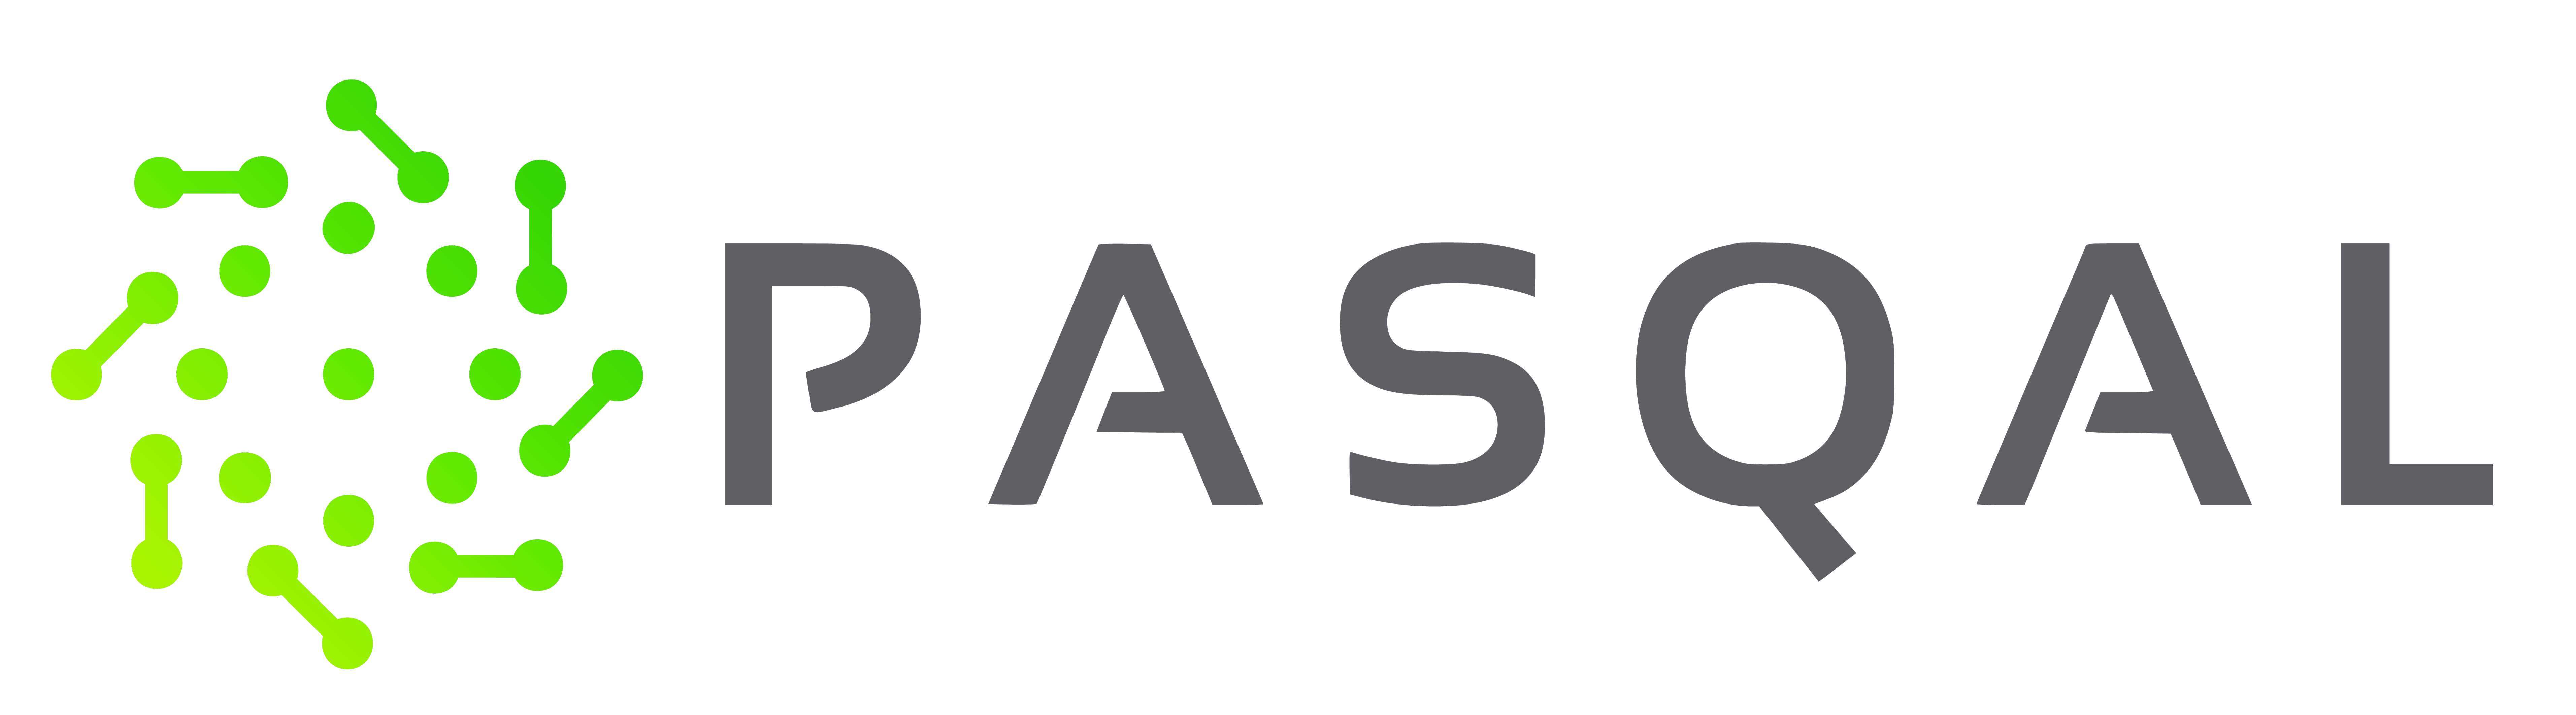
\includegraphics[width=\textwidth]{images/pasqal_logo.png}
             \end{subfigure}
             \hfill
             \begin{subfigure}[b]{0.3\textwidth}
                 \centering
                 
\includegraphics[width=\textwidth]{images/UdeS_logo_rgbHR.png}
             \end{subfigure}
        \end{figure}
    \end{center}
\end{titlepage}

\setcounter{figure}{0}
\tableofcontents
\newpage
\section*{Résumé}
Nous proposons un algorithme adiabatique quantique (QAA) et d'optimisation approximative quantique (QAOA) pouvant résoudre le problème d'un ensemble indépendant maximal d'un graphe. Leurs performances seront comparées à l'implémentation classique actuelle fournie par la librairie \textit{networkx} en python. L'algorithme adiabatique et classique permettra de régler la problématique de l'entreprise québécoise Récupex consistant à replacer leurs cloches récoltant les vêtements usagés dans une distribution optimale pour couvrir l'ensemble du territoire de la ville de Sherbrooke, Québec, Canada. Une recombinaison déterministe pour trouver une approximation d'un ensemble indépendant maximal à l'aide de sous-graphes est aussi présentée. Finalement, il sera déterminé s'il est pertinent actuellement ou dans un futur rapproché d'envisager les méthodes quantiques analogues pour résoudre ce problème.

\section{Introduction}
Récupex est un organisme à but non lucratif dédié à l’insertion socioprofessionnelle des personnes en difficulté d’employabilité. L’organisme gère un vaste réseau de collecte de vêtements, avec une centaine de bacs répartis principalement à Sherbrooke et dans la région de l’Estrie. En partenariat avec des friperies et d’autres organismes communautaires, Récupex contribue activement à la valorisation des textiles usagés, sensibilisant la population aux enjeux environnementaux et recyclant environ 3,5 millions de livres de textiles chaque année.

La gestion des bacs de récupération de vêtements à Sherbrooke présente des défis importants pour Récupex. Les performances varient selon les emplacements en termes de volume de dons, de qualité des textiles et de nuisances (dépôts sauvages, vandalisme). La logistique de collecte demande des ressources significatives (chauffeurs, camions, matériel), rendant l'entretien complexe. Récupex cherche donc à optimiser l'emplacement de ses bacs pour améliorer la collecte, minimiser les nuisances et assurer une gestion efficace des ressources.

\section{Objectifs}
\begin{itemize}
    \item Aider l'organisation Récupex à améliorer leur gestion de bacs de récupération en utilisant différentes approches quantiques.
\item Évaluer la pertinence des approches quantiques lorsqu’elles sont comparées à leur analogue classique.
\item Répondre au plus de conditions de Récupex mentionnées dans la sous-section suivante.
\end{itemize}

\subsection{Conditions de placement des cloches de Récupex}
Récupex applique plusieurs critères pour optimiser l’emplacement de ses bacs de récupération de vêtements, en tenant compte des aspects de couverture, d'accessibilité, et de performance :

\begin{enumerate}
    \item \textbf{Couverture des territoires non desservis} : Récupex cherche à s’assurer que chaque région a accès à un bac, en priorisant les territoires non encore desservis. Cela vise à améliorer l’accessibilité pour tous.

    \item \textbf{Proximité et accessibilité} : Plus un bac est proche des habitants, plus il est accessible et utilisé. Récupex souhaite donc placer les bacs dans des zones faciles d’accès pour maximiser la collecte.

    \item \textbf{Contrôle de la densité de bacs} : Bien qu’il soit important d’avoir des bacs à proximité, Recupex évite de multiplier les bacs dans la même zone pour éviter la redondance et les coûts inutiles.

    \item\textbf{Qualité des dons} : La qualité des vêtements collectés varie selon les quartiers. Dans les zones plus aisées, les vêtements ont tendance à être de meilleure qualité. Cela peut influencer le placement des bacs en fonction des priorités de collecte de qualité. Cette qualité sera exprimé par volume de vêtement reçu en moyenne annuellement par bac. Ce sont les données les plus près de cette condition.

    \item\textbf{Densité de population} : Les secteurs densément peuplés sont plus propices à accueillir plusieurs bacs, car ils génèrent un volume de dons plus élevé. Cette condition ne sera pas considéré dû à un manque de banque de données de densité de population.

    \item\textbf{Pertinence et fonctionnalité des bacs} : Récupex suit la performance de chaque bac (s’il est régulièrement utilisé ou non) pour ajuster leur distribution, en ajoutant, déplaçant ou retirant des bacs selon leur pertinence dans chaque zone.

    \item\textbf{Prendre en considération les autres associations} : Récupex prend en compte la présence d’autres associations, comme Estrie Aide, pour éviter une concurrence directe et mieux répartir les services. Pour notre solution, nous avons pris en considération les bacs de l'entreprise Estrie-Aide.

    \item\textbf{Autorisation pour le placement} : Le placement de chaque bac nécessite une autorisation, et il est plus facile d’obtenir cette autorisation dans des zones où les propriétaires sont plus ouverts au projet.Pour notre solution, nous n'avons pas pris en compte ce résultat puisque nous avons pas un registre de commerçants qui accpeteraient ou non.
\end{enumerate}

\section{Théorie}
\subsection{Graphes}
\subsubsection{Introduction aux graphes}
Un graphe est un objet mathématique très utile lorsqu'une carte doit être représentée dans un ordinateur \cite{mackaness_use_1993}\cite{riaz_applications_2011}. Ce dernier est représenté par un ensemble $G=(V,E)$ où V est un ensemble de sommets et E l'ensemble des arrêtés du graphe. Un sommet est un point dans l'espace qui sera connecté à un autre grâce à une arrête. Voici la manière usuelle de représenter un graphe.

\begin{figure}[H]
    \centering
        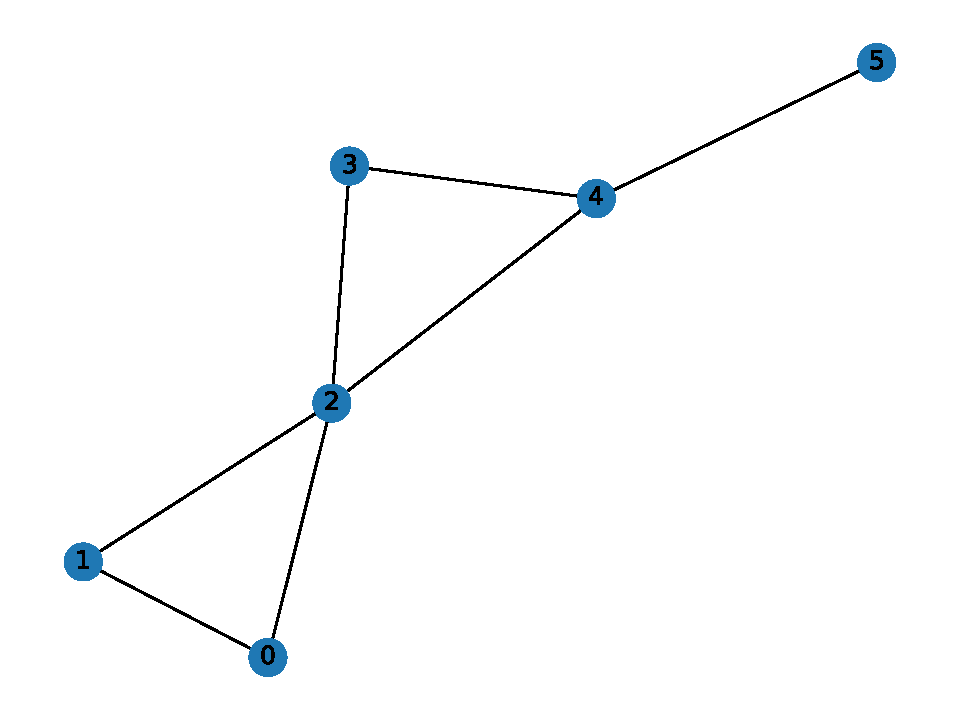
\includegraphics[width=0.45\linewidth]{images/graphe_MIS_exemple.pdf}
        \caption{Exemple de graphe}
    \label{graph_exemple}
\end{figure}

Par contre, l'utilisation de graphes par disques unitaires sera plus appropriée pour le projet. Dans ce type de graphe, on note la position des sommets dans l'espace et non leur relation entre eux. Pour définir les opérations, nous traçons un disque de rayon arbitrairement défini plutôt auparavant. Ensuite, si deux cercles de deux sommets distincts se croisent, il y a alors une interaction entre ces deux sommets. Voici la comparaison entre un graphe de disque unitaire et son analogue de représentation plus «classique». 
\begin{figure}[H]
    \centering
        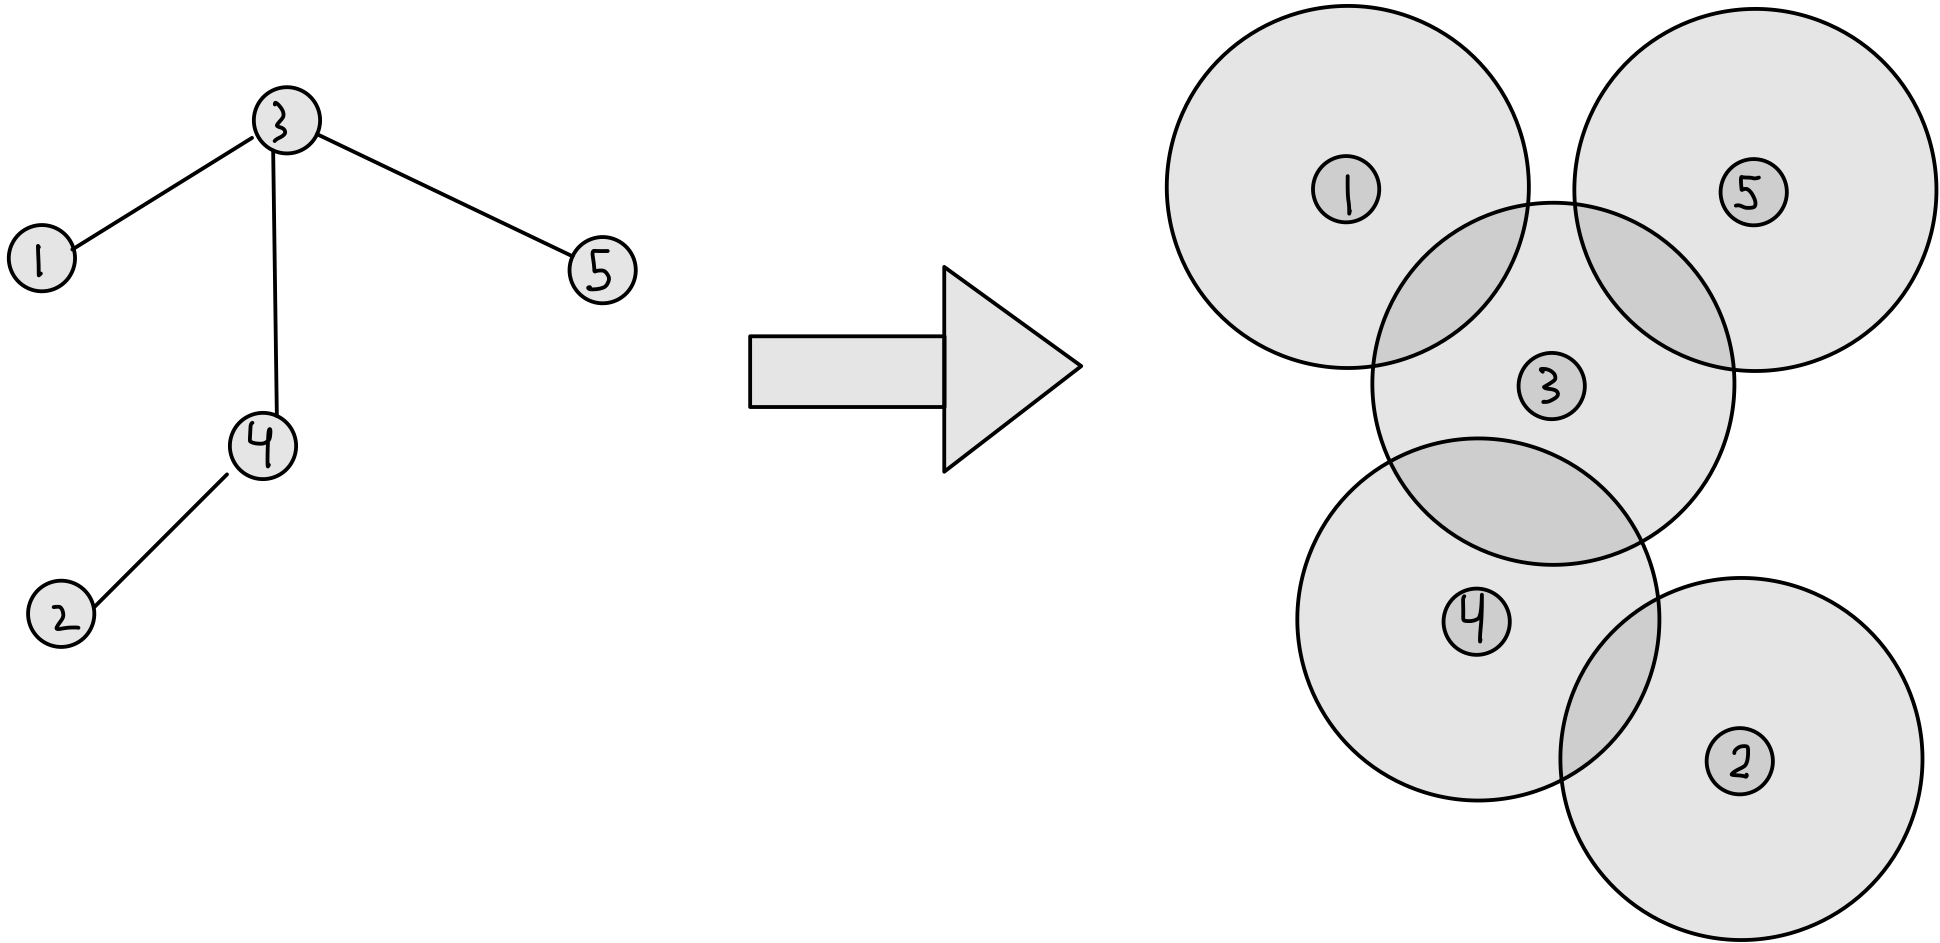
\includegraphics[width=0.45\linewidth]{images/disk_ex.jpg}
        \caption{Exemple de graphes à disques unitaires.}
    \label{disk_example}
\end{figure}
\subsubsection{Ensemble indépendant maximal}
Un ensemble indépendant maximal est un ensemble de sommets qui ne sont pas connectés par une arête. Cet ensemble doit contenir le plus de sommets possible afin d'être complet. Par exemple, le graphe de la figure \ref{graph_exemple} comporte 6 noeuds et son ensemble indépendant maximal en comporte 3.
 
Il peut y avoir plusieurs ensembles indépendants maximaux pour un seul graphe comme c'est le cas avec le graphe précédent. Les ensembles correspondants seraient \{1, 4, 6\} et \{2, 4, 6\} comme illustrés par la figure \ref{MIS_exemple}.

\begin{figure}[H]
    \centering
    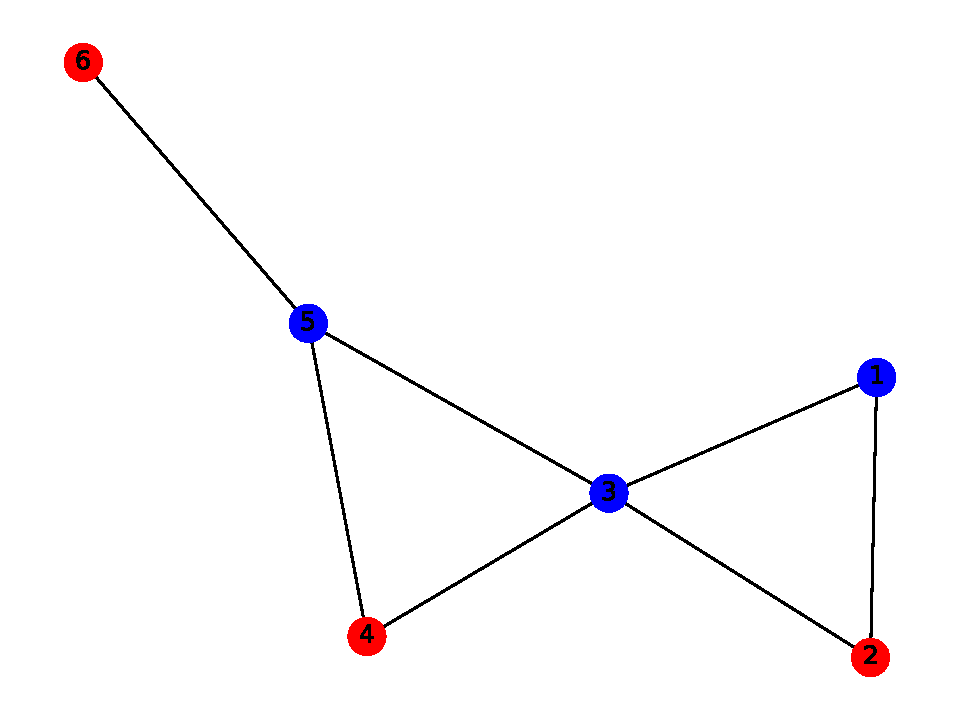
\includegraphics[width=0.4\linewidth]{images/graphe_MIS_1.pdf}
    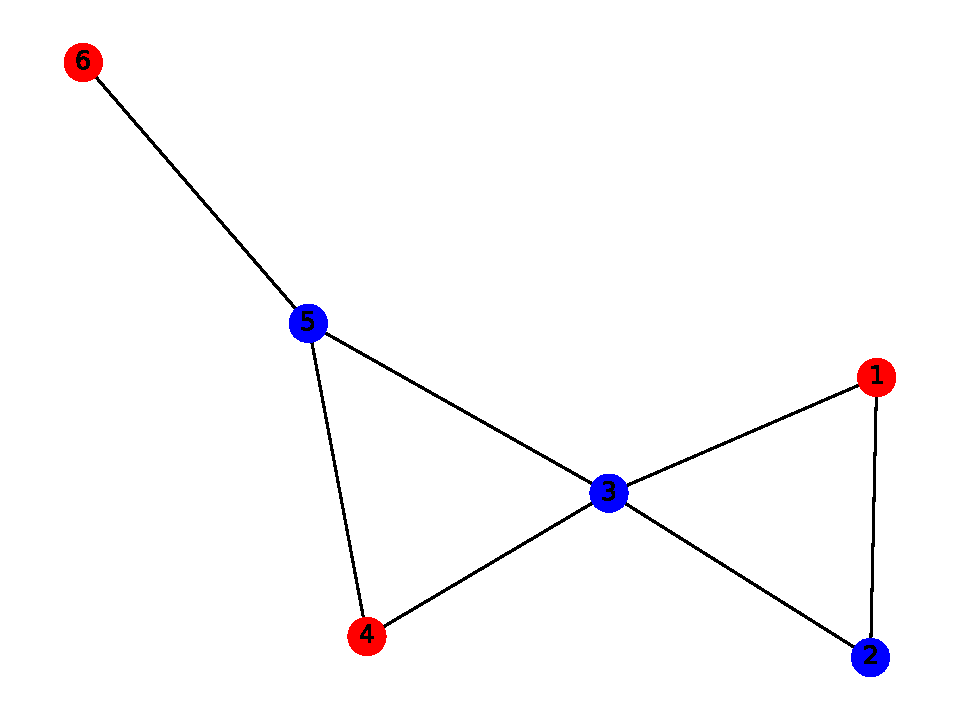
\includegraphics[width=0.4\linewidth]{images/graphe_MIS_2.pdf}
    \caption{Ensembles indépendants maximaux pour le graphe de la figure 1.}
    \label{MIS_exemple}
\end{figure}



\subsection{Grapher Sherbrooke}
Récupex se doit de couvrir l'ensemble de Sherbrooke au meilleur de ses possibilités avec ses 60 bacs. Il faut alors trouver une manière de représenter la ville dans l'ordinateur quantique. Pour ce faire, nous allons utiliser un graphe. 

Pour utiliser cet objet mathématique dans notre problématique, nous allons représenter tous les emplacements possibles des bacs par un sommet du graphe. Ces emplacements ont été définis grâce à une base de données des édifices commerciaux et industriels de la ville de Sherbrooke \cite{noauthor_repertoire_nodate}. Nous avons raffiné cette base de données en gardant seulement les commerces, les institutions et lieux publics. En effet, les bacs ne peuvent pas être situés sur un terrain résidentiel ou industriel pour encourager les dons. Nous allons représenter le graphe de la ville selon un graphe de disque unitaire. Les sommets du graphe sont donc ces emplacements possibles et nous notons leur position dans l'espace par leur longitude sur l'axe des x et leur latitude sur l'axe des y. Par la suite, pour définir les arrêtes du graphe, il suffit de définir un rayon pour  lequel les endroits possibles sont connectés. Par la suite, un algorithme d'ensemble indépendant maximal pourra être utilisé pour faire ressortir le nombre maximal d'emplacements qui ne sont pas trop proches des autres et de bacs actuels pour mettre des bacs.


 \begin{figure}[H]
    \centering
        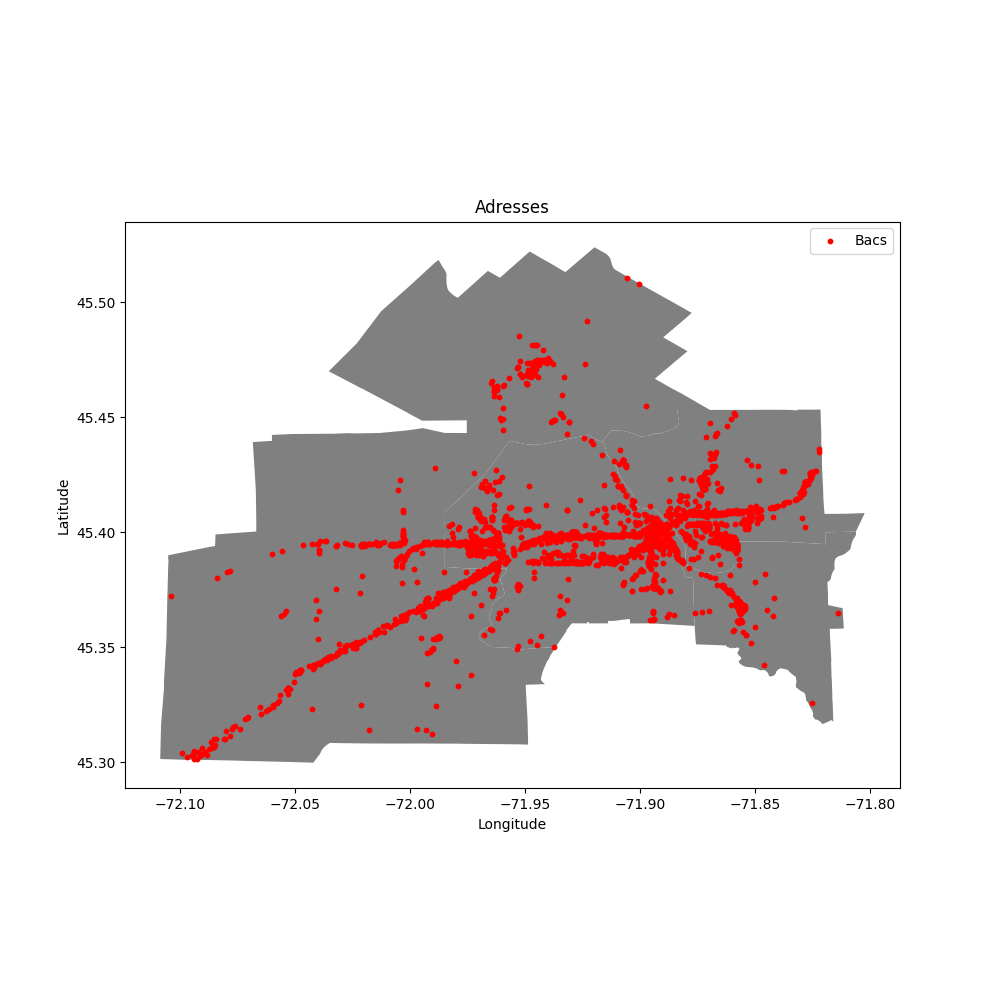
\includegraphics[width=0.5\linewidth]{images/commerces.png}
        \caption{Emplacements possibles des bacs dans la ville de Sherbrooke}
    \label{bacs_possibles_total}
\end{figure}


\subsection{Ordinateur quantique à atome neutre}
L'ordinateur quantique à atome neutre utilisée sera employé comme un ordinateur analogue. Pour ce projet, nous utiliserons les appareils développés par Pasqal \cite{browaeys_quantum_2019}. Le qubit de cet ordinateur quantique est un atome de Rydberg. Cet atome peut se trouver dans l'état fondamental $\ket{g}$ ou dans son état excité $\ket{R}$ \cite{noauthor_learn_nodate}. L'intrication entre les qubits est créée à l'aide du rayon de blocage de Rydberg. Quand un atome atteint l'état $\ket{R}$, les atomes plus près de ce dernier qu'une distrance prédéfinie (le rayon de blocage) on besoin de beaucoup plus d'énergie pour qu'ils atteigent aussi l'état $\ket{R}$. La première étape du calcul quantique est de créer un registre contenant des atomes à certaines positions afin de représenter notre problème dans l'ordinateur. Pour ce projet, nous ne considèrerons seulement que des registres en deux dimensions. Des pinces optiques sont positionnées \cite{browaeys_pinces_2016} aux endroits déterminés afin de capturer les atomes. Puisque le taux de capture des pinces optiques est d'environ 55\% \cite{muldoon_control_2012}, le double du nombre de pinces optiques est placé dans le registre. Après la capture des atomes, on vérifie leurs positions pour ensuite les replacer un par un afin de créer le registre voulu. Tout ce processus est fait directement par Pulser \cite{silverio_pulser_2022} lors de la création d'un registre. Le calcul quantique se fait à l'aide d'un pulse. Le pulse peut avoir plusieurs formes et atteint une certaine valeur maximale $\Omega_{max} $ qui définit le rayon de blocage.  Les atomes se tenant à l'intérieur de ce cercle demandent une valeur de désaccord beaucoup plus grande afin de s'exciter. Le désaccord noté $\delta$ est une valeur qui influe sur le pulse envoyé. Un désaccord négatif pousse les atomes dans l'état fondamental alors qu'un désaccord positif pousse les atomes dans l'état excité. Le désaccord doit donc être négatif au début afin d'initialiser les atomes dans leur état fondamental. La valeur augmente au fur et à mesure du calcul et atteint une valeur positive afin de pousser les atomes à l'état excité. Durant le pulse, certains atomes vont s'exciter et seront éjectés du registre avant la mesure. On mesure donc par fluorescence les atomes dans l'état fondamental présents dans le registre à la suite du pulse pour déduire que les atomes manquants sont les atomes qui ont été excités. Cette mesure est aussi effectuée par Pulser directement. Ainsi, pour utiliser l'ordinateur quantique à atome neutre de Pasqal, l'utilisateur doit simplement définir une séquence contenant la forme du registre et le Pulse en fonction du temps. 


\subsection{Trouver l'ensemble indépendant maximal à l'aide de l'ordinateur quantique à atome neutre}
Le problème np complet \cite{tarjan_finding_1977} qu'est de trouver l'ensemble maximal indépendant (MIS) d'un graphe géométrique peut être résolu grâce à la technologie d'ordinateurs à atomes neutres \cite{dettmann_random_2016}. Deux méthodes trouvant les MIS seront proposés, l'algorithme quantique adiabatique ou bien l'algorithme d'optimisation approximative quantique \cite{ebadi_quantum_2022}.

\subsubsection{Algorithme quantique adiabatique}
La première étape est de créer le registre en fonction du graphe. La clé est de ne considérer que les interactions entre les noeuds du graphe. Ces interactions sont reliées directement au rayon de blocage dans le registre. On doit alors positionner les atomes afin de créer le graphe à disque unitaire en fonction du graphe en entrée. Cette étape est la plus complexe à réaliser en terme d'implémentation. Le registre doit respecter des contraintes physique de placement entre les atomes en fonction de l'appareil utilisé. Il est donc difficle de créer un bon registre pour un graphe géométrique en général. Pour simplifier la création des registres, nous avons utilisé un algorithme qui sépare les graphes en composantes connexes, puisque l'ensemble indépendant maximal d'un graphe contenant plusieurs composantes connexes est tout simplement la somme des ensembles indépendants maximals des composantes connexes. Il ne reste plus qu'à construire un pulse avec une valeur de $\Omega_{max}$, appelée fréquence de Rabi, en fonction du rayon de blocage souhaité. Il doit être appliqué à tout les atomes du registre. Le pulse doit valoir 0 au départ et atteindre $\Omega_{max}$ avant de redescendre à 0. Plusieurs types de pulse sont possibles. La figure \ref{pulse_exemple} présente un exemple de pulse à appliquer. Les pulse utilisés sont présentés à la section \ref{pulse_opt}.
\begin{figure}[H]
    \centering
    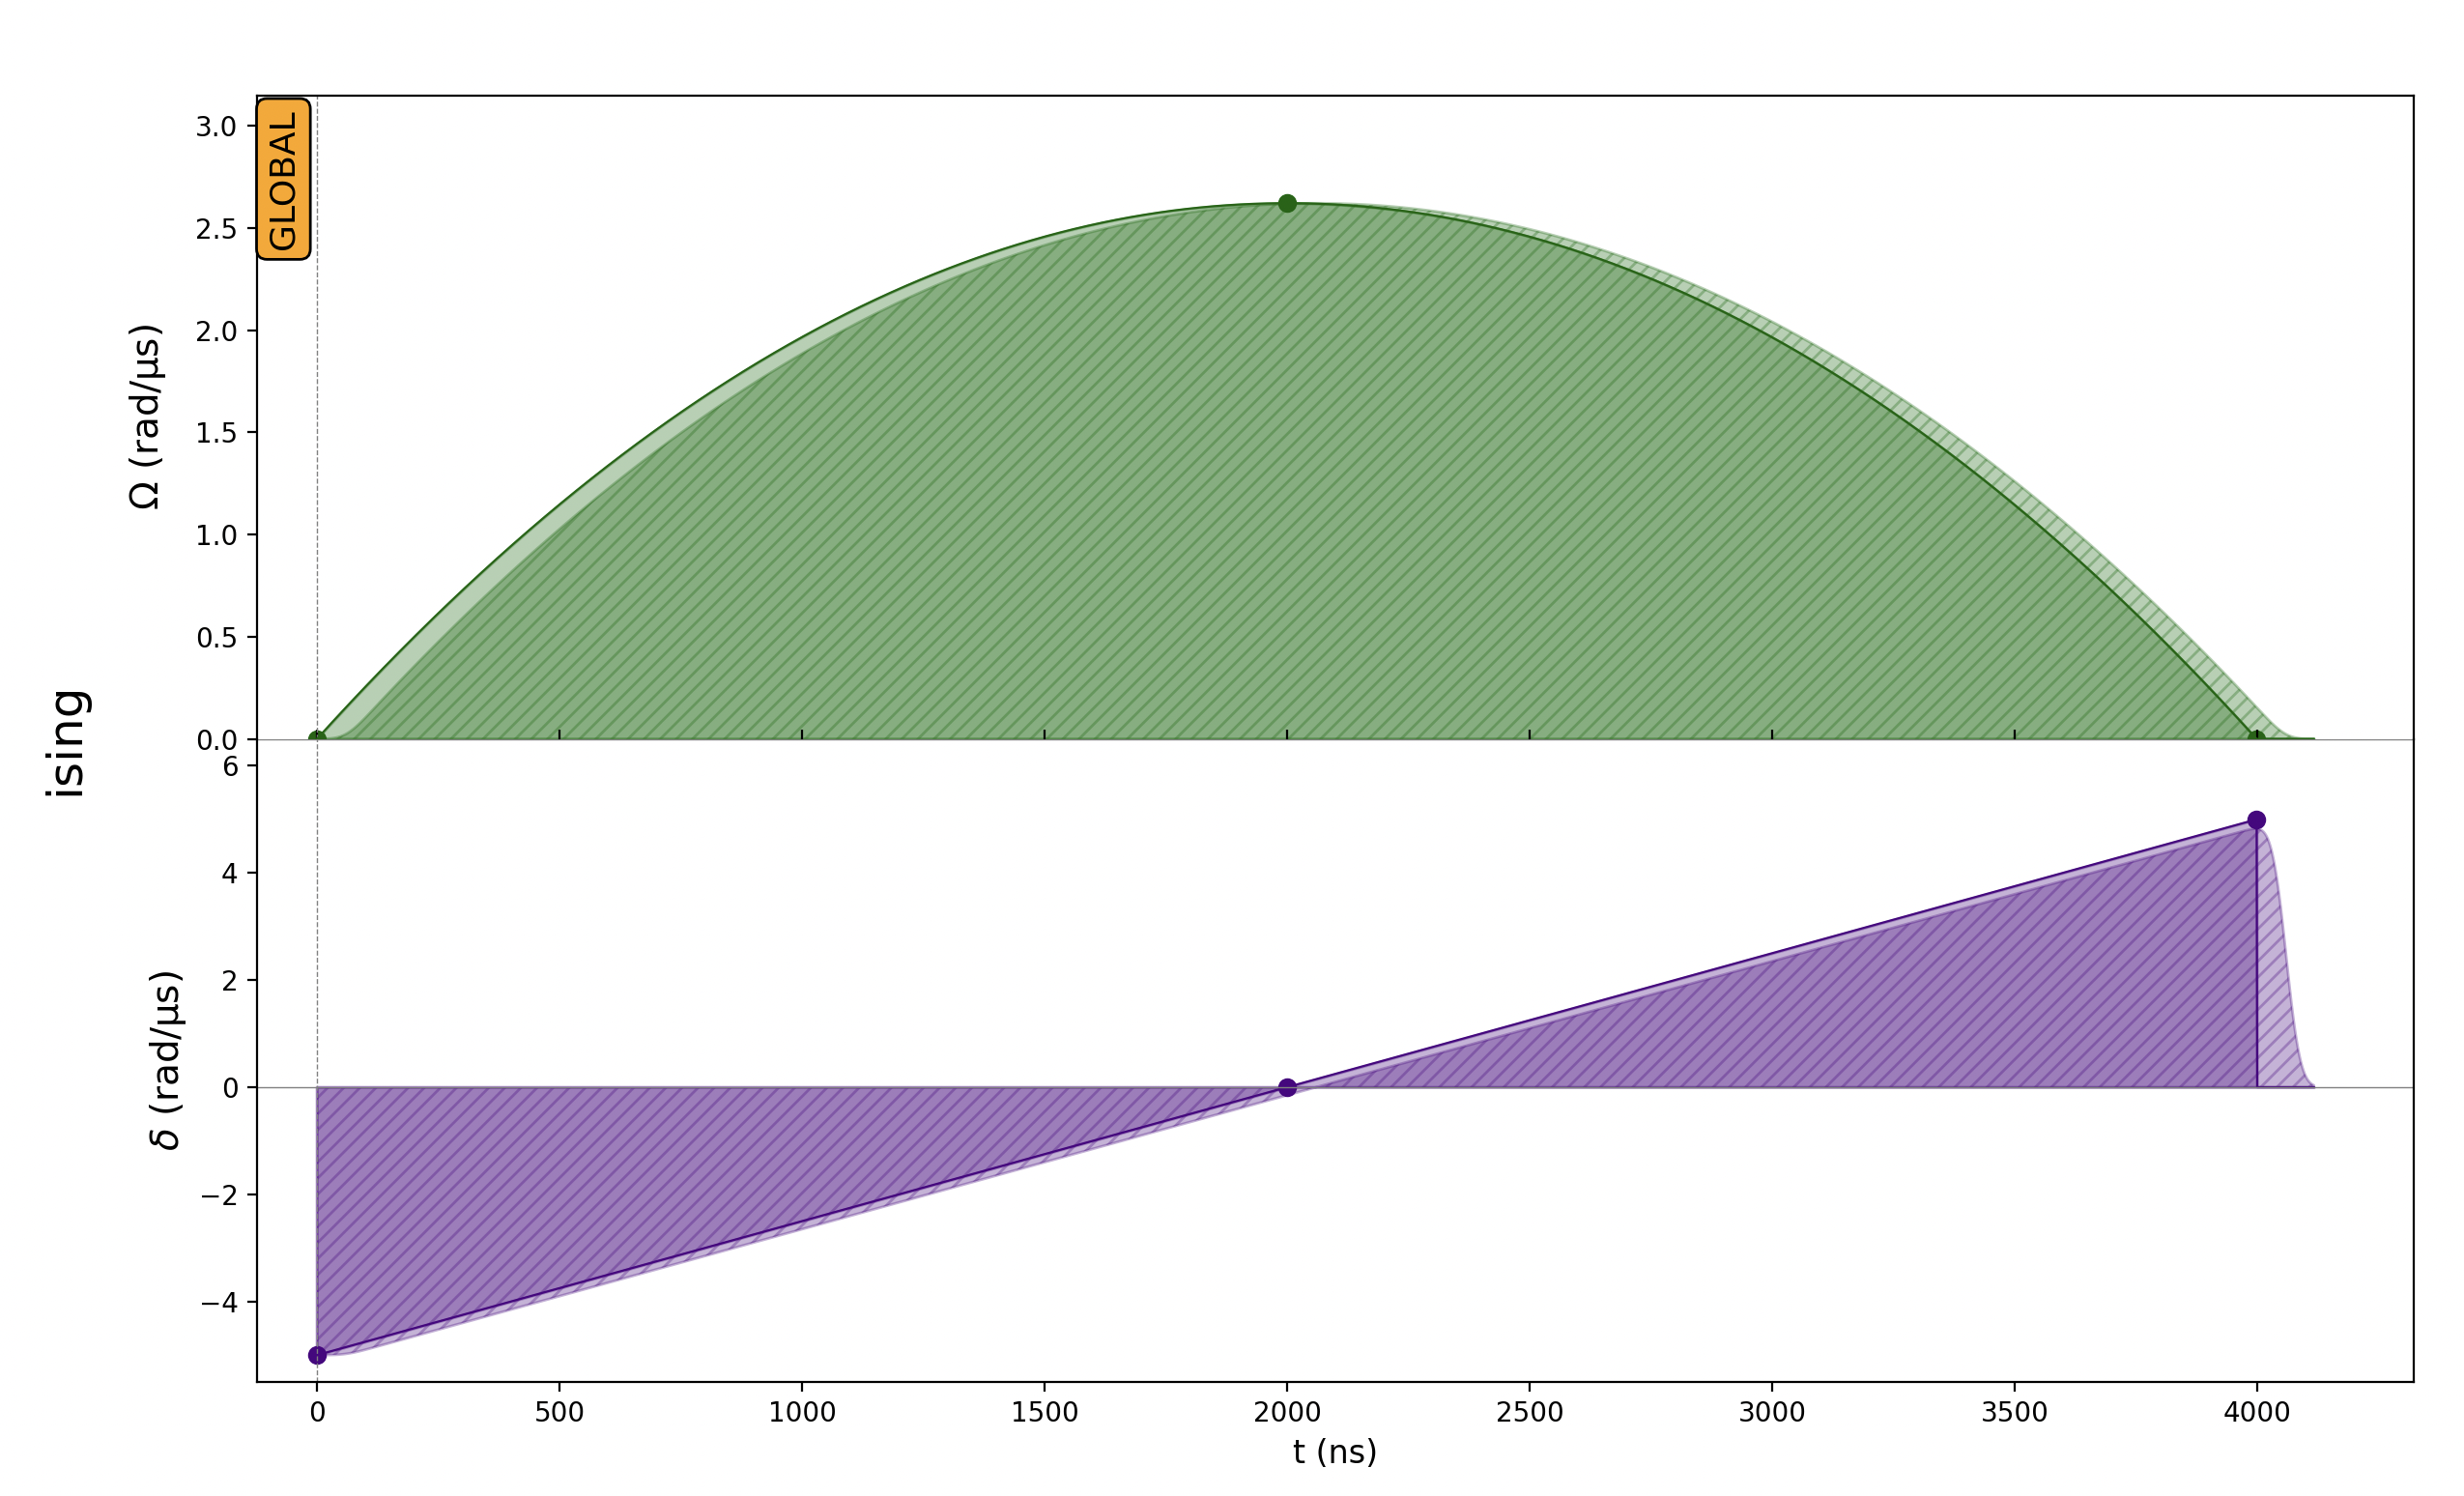
\includegraphics[width = 0.6\linewidth]{images/pulse_exemple.png}
    \caption{Exemple de Pulse adiabatique}
    \label{pulse_exemple}
\end{figure}
L'algorithme quantique adiabatique tente de transformer un hamiltonien initial en un hamiltonien final en lui appliquant le pulse de la plus longue durée possible. L'hamiltonien initial du système est ici représenté par le registre initial créé. En lui appliquant le pulse, on retrouve l'hamiltonien final qui encode la solution. En fait, comme vu précédemment, les atomes ayant une distance entre eux inférieur au rayon de blocage ne peuvent pas être dans l'état excité en même temps. Puisque les sommets qui sont liés par une arête dans le graphe sont à des positions contenus dans le rayon de blocage dans le registre, un seul des deux va pouvoir s'exciter. Ainsi, l'hamiltonien final ne contiendra que des atomes excités qui forment un ensemble indépendant maximal. Le calcul quantique ne donne pas toujours le même résultat et ne donne pas toujours l'ensemble indépendant maximal. En fait, puisque le temps le temps d'application du pulse est limité, le retour optimal de l'ordinateur n'est pas toujours observé. Si le pulse pouvait s'appliquer beaucoup plus longtemps, il nous faudrait théoriquement un seul calcul pour trouver directement l'ensemble indépendant maximal par le théorème adiabatique \cite{amin_consistency_2009}. Le calcul est donc effectué un certain nombre de fois afin d'obtenir un histogramme contenant plusieurs résultats. Les résultats qui  le ont la plus grande fréquence de retour dans l'histogramme sont théoriquement des ensembles indépendants maximals. Par exemple, on pourrait prendre le graphe de la figure 1 et trouver l'ensemble indépendant maximal avec les étapes expliquées ci-dessus afin d'obtenir le registre et l'histogramme de la figure \ref{QMIS_exemple}.
\begin{figure}[H]
    \centering
    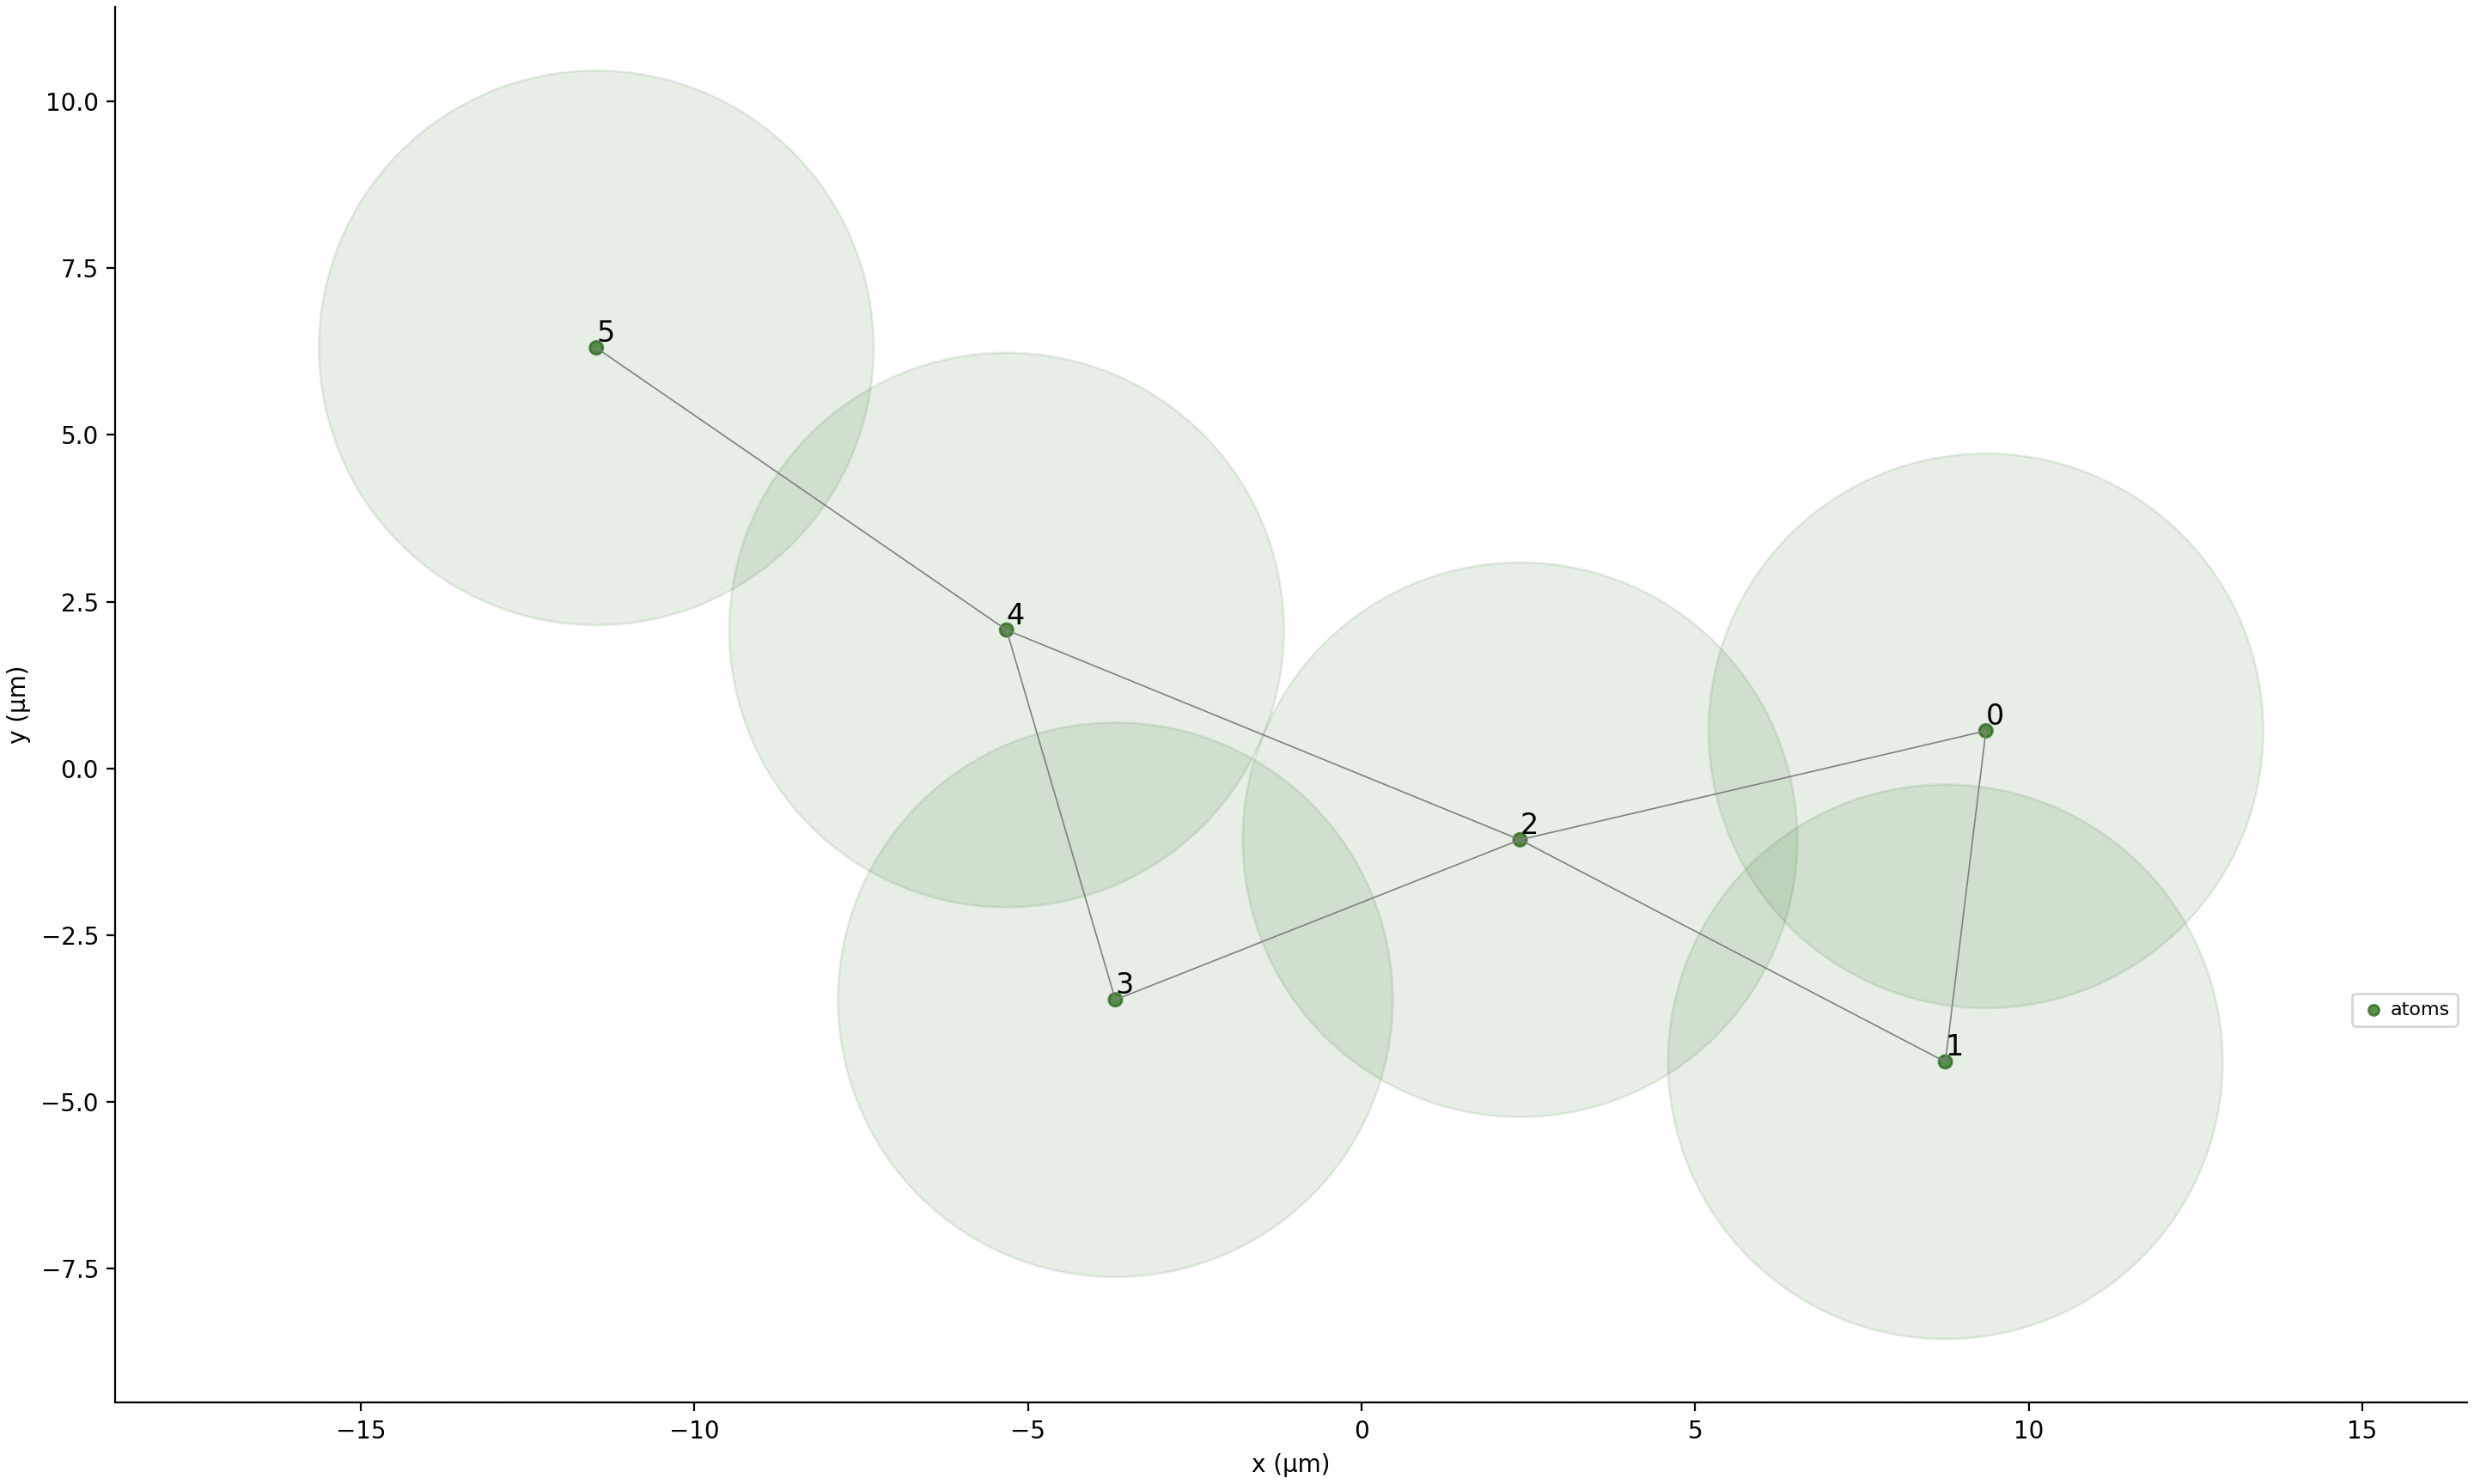
\includegraphics[width = 0.48\linewidth]{images/registre_exemple.png}
    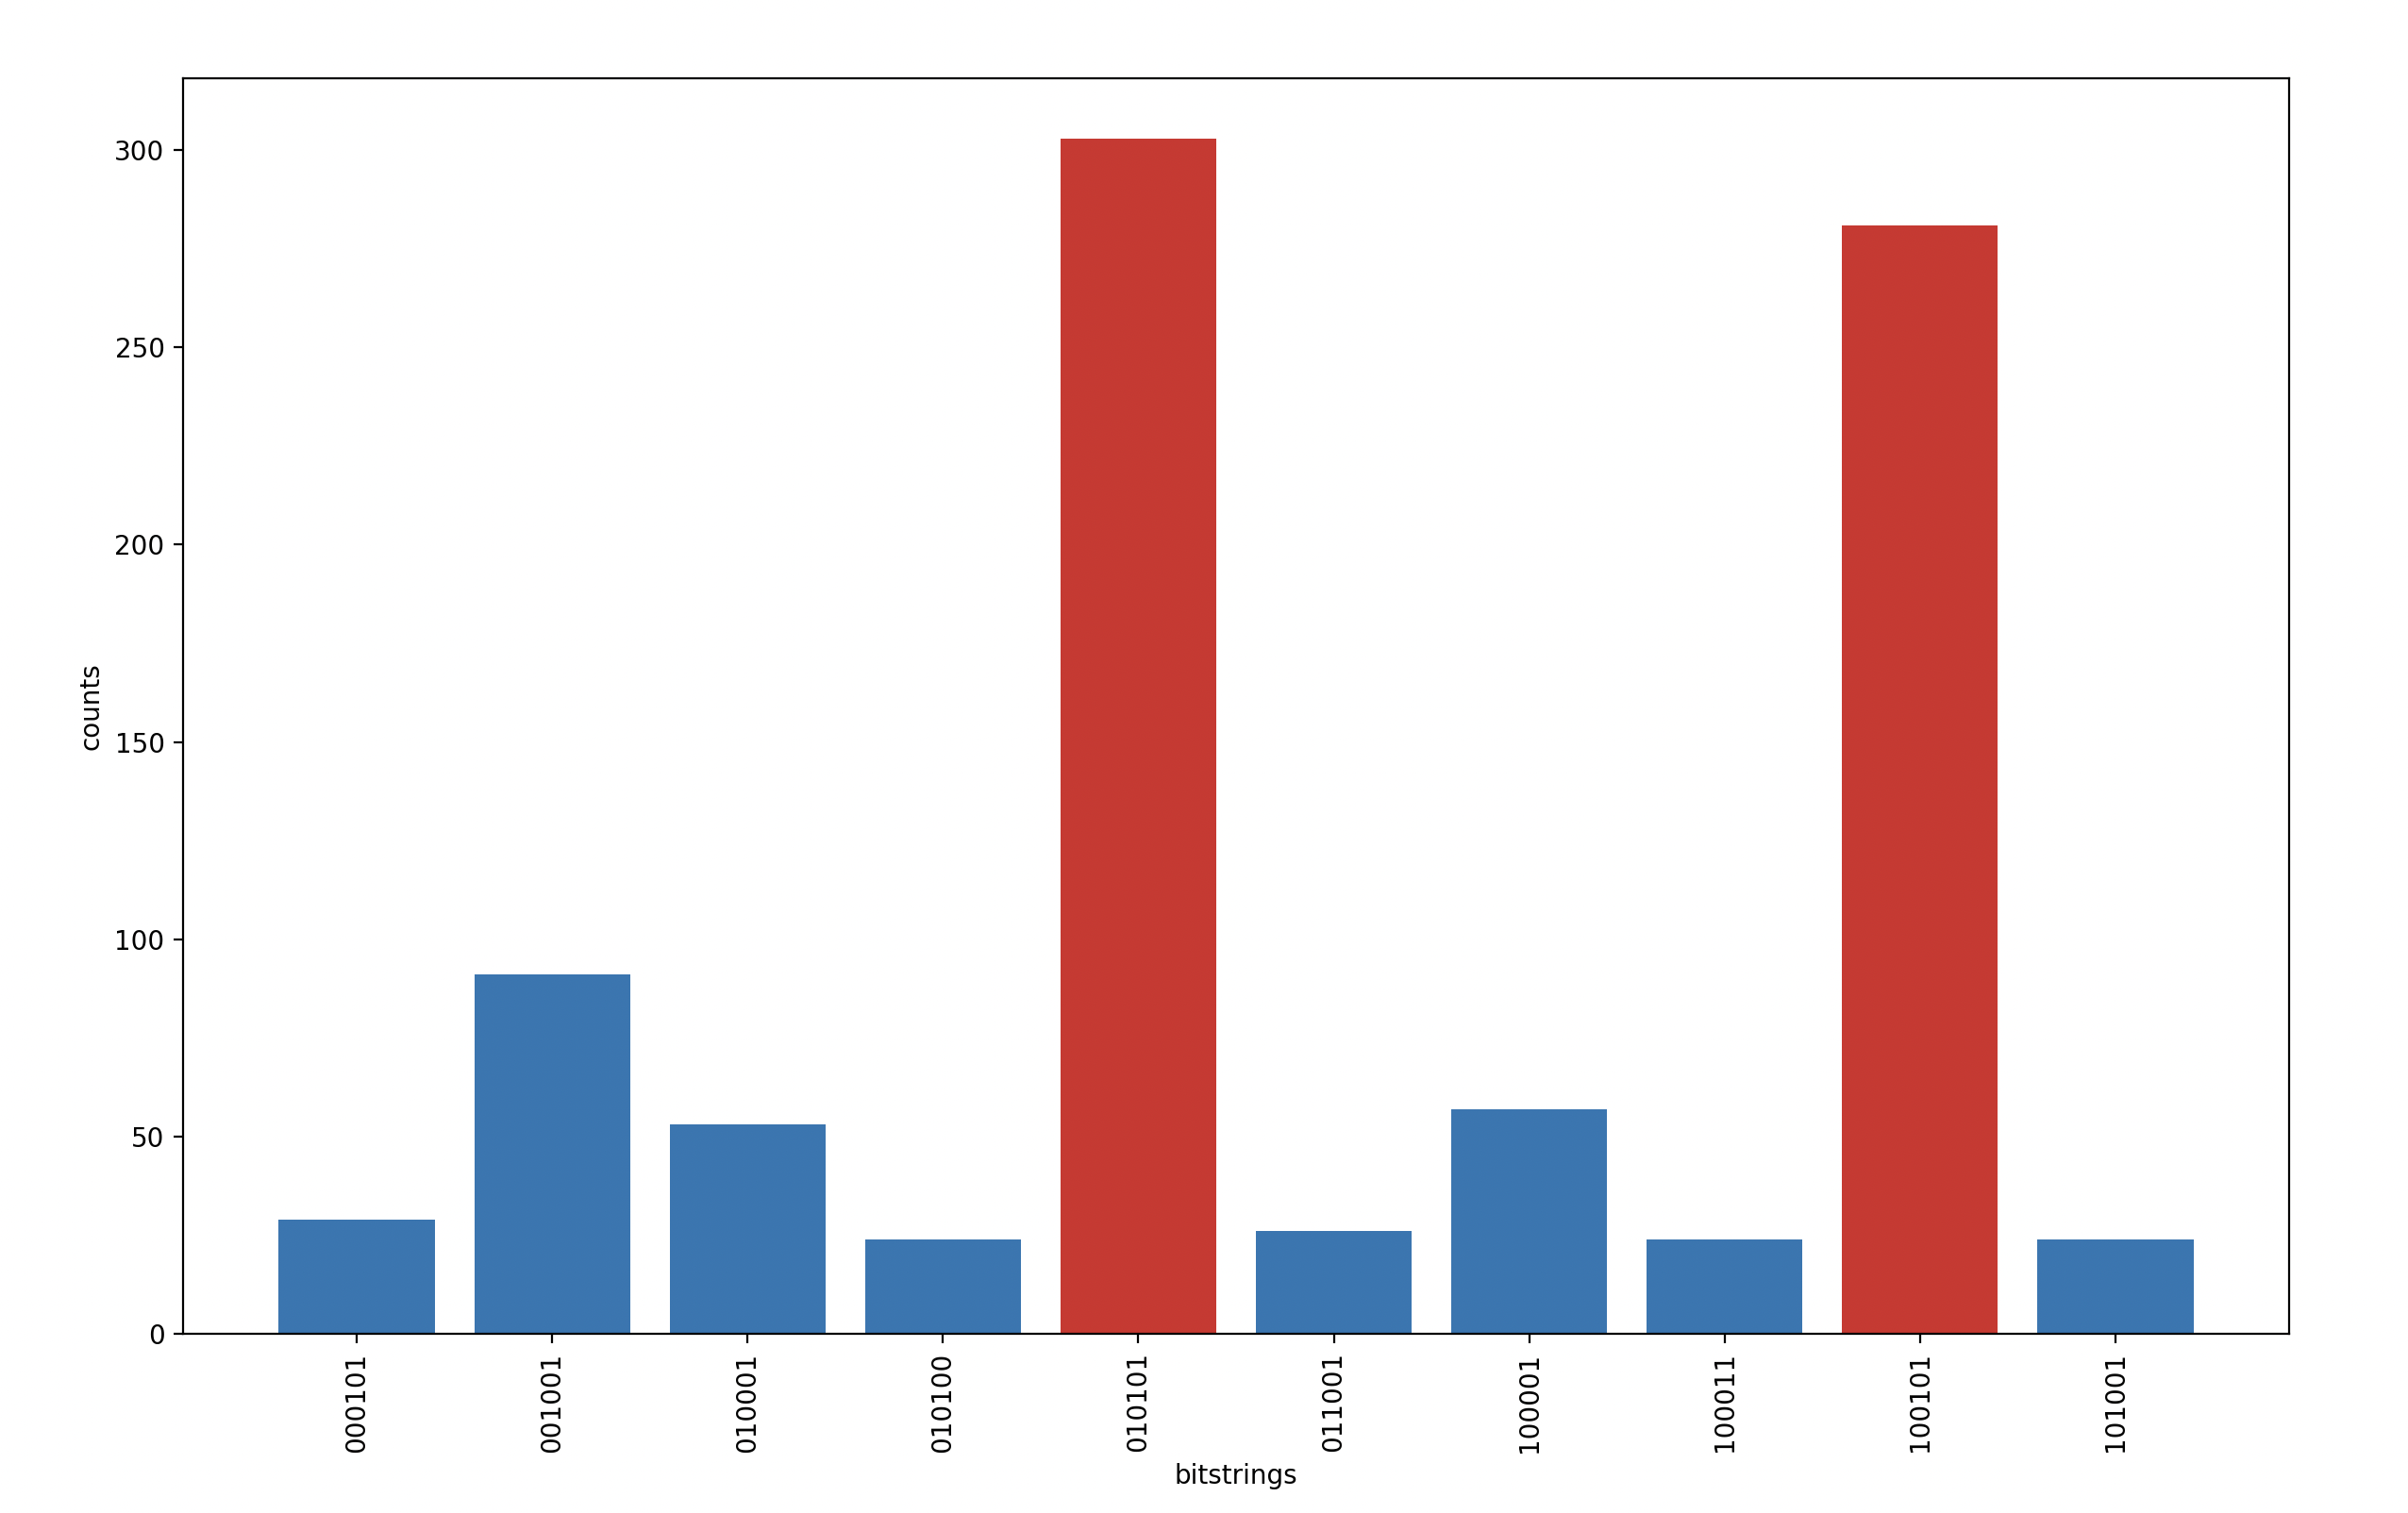
\includegraphics[width=0.49\linewidth]{images/histo_qaa_exemple.png}
    \caption{Registre quantique et l'histogramme associé à ce registre après 1000 tentatives}
    \label{QMIS_exemple}
\end{figure}
    
Les deux solutions suivantes sont donc les mis rétournés: \{0, 3, 5\}, \{1, 3, 5\}. Elles correspondent bien aux deux solutions admises du graphe de la figure \ref{MIS_exemple}.


%Dans le cadre de notre projet avec Récupex, nous avons utilisé une approche d'un ordinateur à atomes neutres pour résoudre un problème d'optimisation combinatoire, qui est de trouver le maximum independant set (MIS) dans notre graphe. Les ordinateurs à atomes neutres, tels que ceux développés par Pasqal, manipulent des qubits representées par des atomes de Rydberg, dont l'intrication repose sur le phénomène de blocage de Rydberg. Cette méthode permet de modeliser les graphes ou les qubits interagissent en fonction de leurs emplacements dans l'espace et des pulses appliqués.
%D'autre part le problème du MIS nous permet de sélectionner les emplacements qui maximisent l'efficacité de collecte tout en minimisant les conflits potentiels dans l'emplacement des bacs (comme la proximité excessive). En utilisant une approche de calcul analogue, nous pouvons tirer parti des propriétes physiques du système quantique pour explorer rapidement et efficacement les résultats possibles, ce qui nous aidera a trouver les configurations optimales répondant aux critères et objectifs de performance de Récupex 

\subsubsection{Algorithme d'optimisation approximative quantique} 
 
 L'algorithme d'optimisation approximative quantique (\textit{QAOA}) est une méthode largement utilisée pour résoudre des problèmes d'optimisation combinatoire tels que le problème de l'ensemble indépendant maximal \cite{farhi_quantum_2014}. Le QAOA utilise des circuits quantiques pour approximer les solutions optimales des problèmes. Il repose sur la définition de deux hamiltoniens : l'hamiltonien de coût ($H_c$), dont l'état fondamental encode la solution du problème d’optimisation, et l'hamiltonien de mélange ($H_m$) , conçu pour explorer l'espace des états quantiques. 
 L'algorithme alterne ensuite l'application de ces deux hamiltoniens sur un état initial. À chaque étape, l'hamiltonien de coût est appliqué pendant un temps $\alpha$, et l'hamiltonien de mélange pendant un temps $\beta$.  Ces paramètres $\alpha$ et $\beta$ sont ensuite optimisés à l'aide de méthodes d'optimisation classique pour maximiser la probabilité de mesurer une solution optimale.
 Avec un nombre élevé d'étapes ( représentées par la profondeur p ), le QAOA peut théoriquement s'approcher de plus en plus de la solution optimale. Il s'impose donc comme une technique prometteuse pour aborder des problèmes complexes, notamment ceux liés aux graphes, ainsi que des problèmes industriels et logistiques.

 L'algorithme QAOA alterne entre deux pulses sur \( p \) couches, chacun représentant un Hamiltonien spécifique. Le premier, appelé \textit{Hamiltonien de mélange} (\textit{mixing Hamiltonian}), est paramétré par \( \Omega \) et \( T_{\text{mixer}} \) et est conçu pour permettre l'exploration de l'espace des solutions. Le second, appelé \textit{Hamiltonien de coût} (\( H_q \)), encode la fonction objectif à optimiser. Ce deuxième pulse, paramétré par \( \Omega \) et \( T_{\text{cost}} \), oriente l'évolution du système vers des états correspondant aux solutions optimales.


\subsection{Ensemble maximal indépendant en sous-graphe}
Sachant que le simulateur quantique ne peut traiter que des problèmes à 25 atomes (équivalent à un graphe d'au plus 25 sommets que l'on tente de trouver l'ensemble indépendant maximal), un graphe contenant beaucoup plus de point doit être traité en sous-instance de graphe. La première étape consiste à employer l'algorithme METIS \cite{karypis_multilevelk-way_1998}. Il permet de séparer un graphe en n sous-graphes contenant environ le même nombre de sommets tout en minimisant le nombre d'arrêtes perdues dans la somme des sous-graphes. Cet algorithme sera utile puisqu'il permet de créer juste le nombre d'instances de sous-graphe nécessaire pour faire le plus de calcul quantique possible tout en gardant le plus d'information possible. 

Par la suite, pour recombiner les ensembles indépendants maximals des sous-graphes, nous allons effectuer un algorithme permettant de fusionner une paire de ceux-ci. Selon Michael Blondin, professeur en algorithmie à l'Université de Sherbrooke \cite{blondin_entretien_2024}, il est possible de créer un ensemble indépendant maximal rapidement en prenant simplement les noeuds impliqués dans les MIS et la connexion entre les deux sous-graphes. Autrement dit, en créant le graphe reliant les points du MIS des sous-graphes A et B selon les arêtes du graphe initial, il est possible de trouver le MIS de ce nouveau graphe rapidement. Les sommets qui n'ont pas d'arêtes reliant un sommet de l'autre sous-graphe ne sont pas inclus dans ce nouveau graphe.

Le graphe obtenu est acyclique et est nommé forêt. Il est possible de trouver l'ensemble maximal indépendant de ce type de graphe par un algorithme classique inspiré de la programmation dynamique. Même s'il n'existe pas de garantie que la solution ne sera pas un ensemble indépendant maximal, il restera tout de même indépendant et cette recombinaison permet d'utiliser le simulateur quantique avec une bonne approximation de la réponse.

\section{Méthodologie}

\subsection{Comparer les méthodes trouvant le MIS}
\subsubsection{Choisir la méthode quantique la plus prometteuse}
L'algorithme adiabatique et d'optimisation approximative seront testés sur le registre suivant: 

\begin{figure}[H]
    \centering
    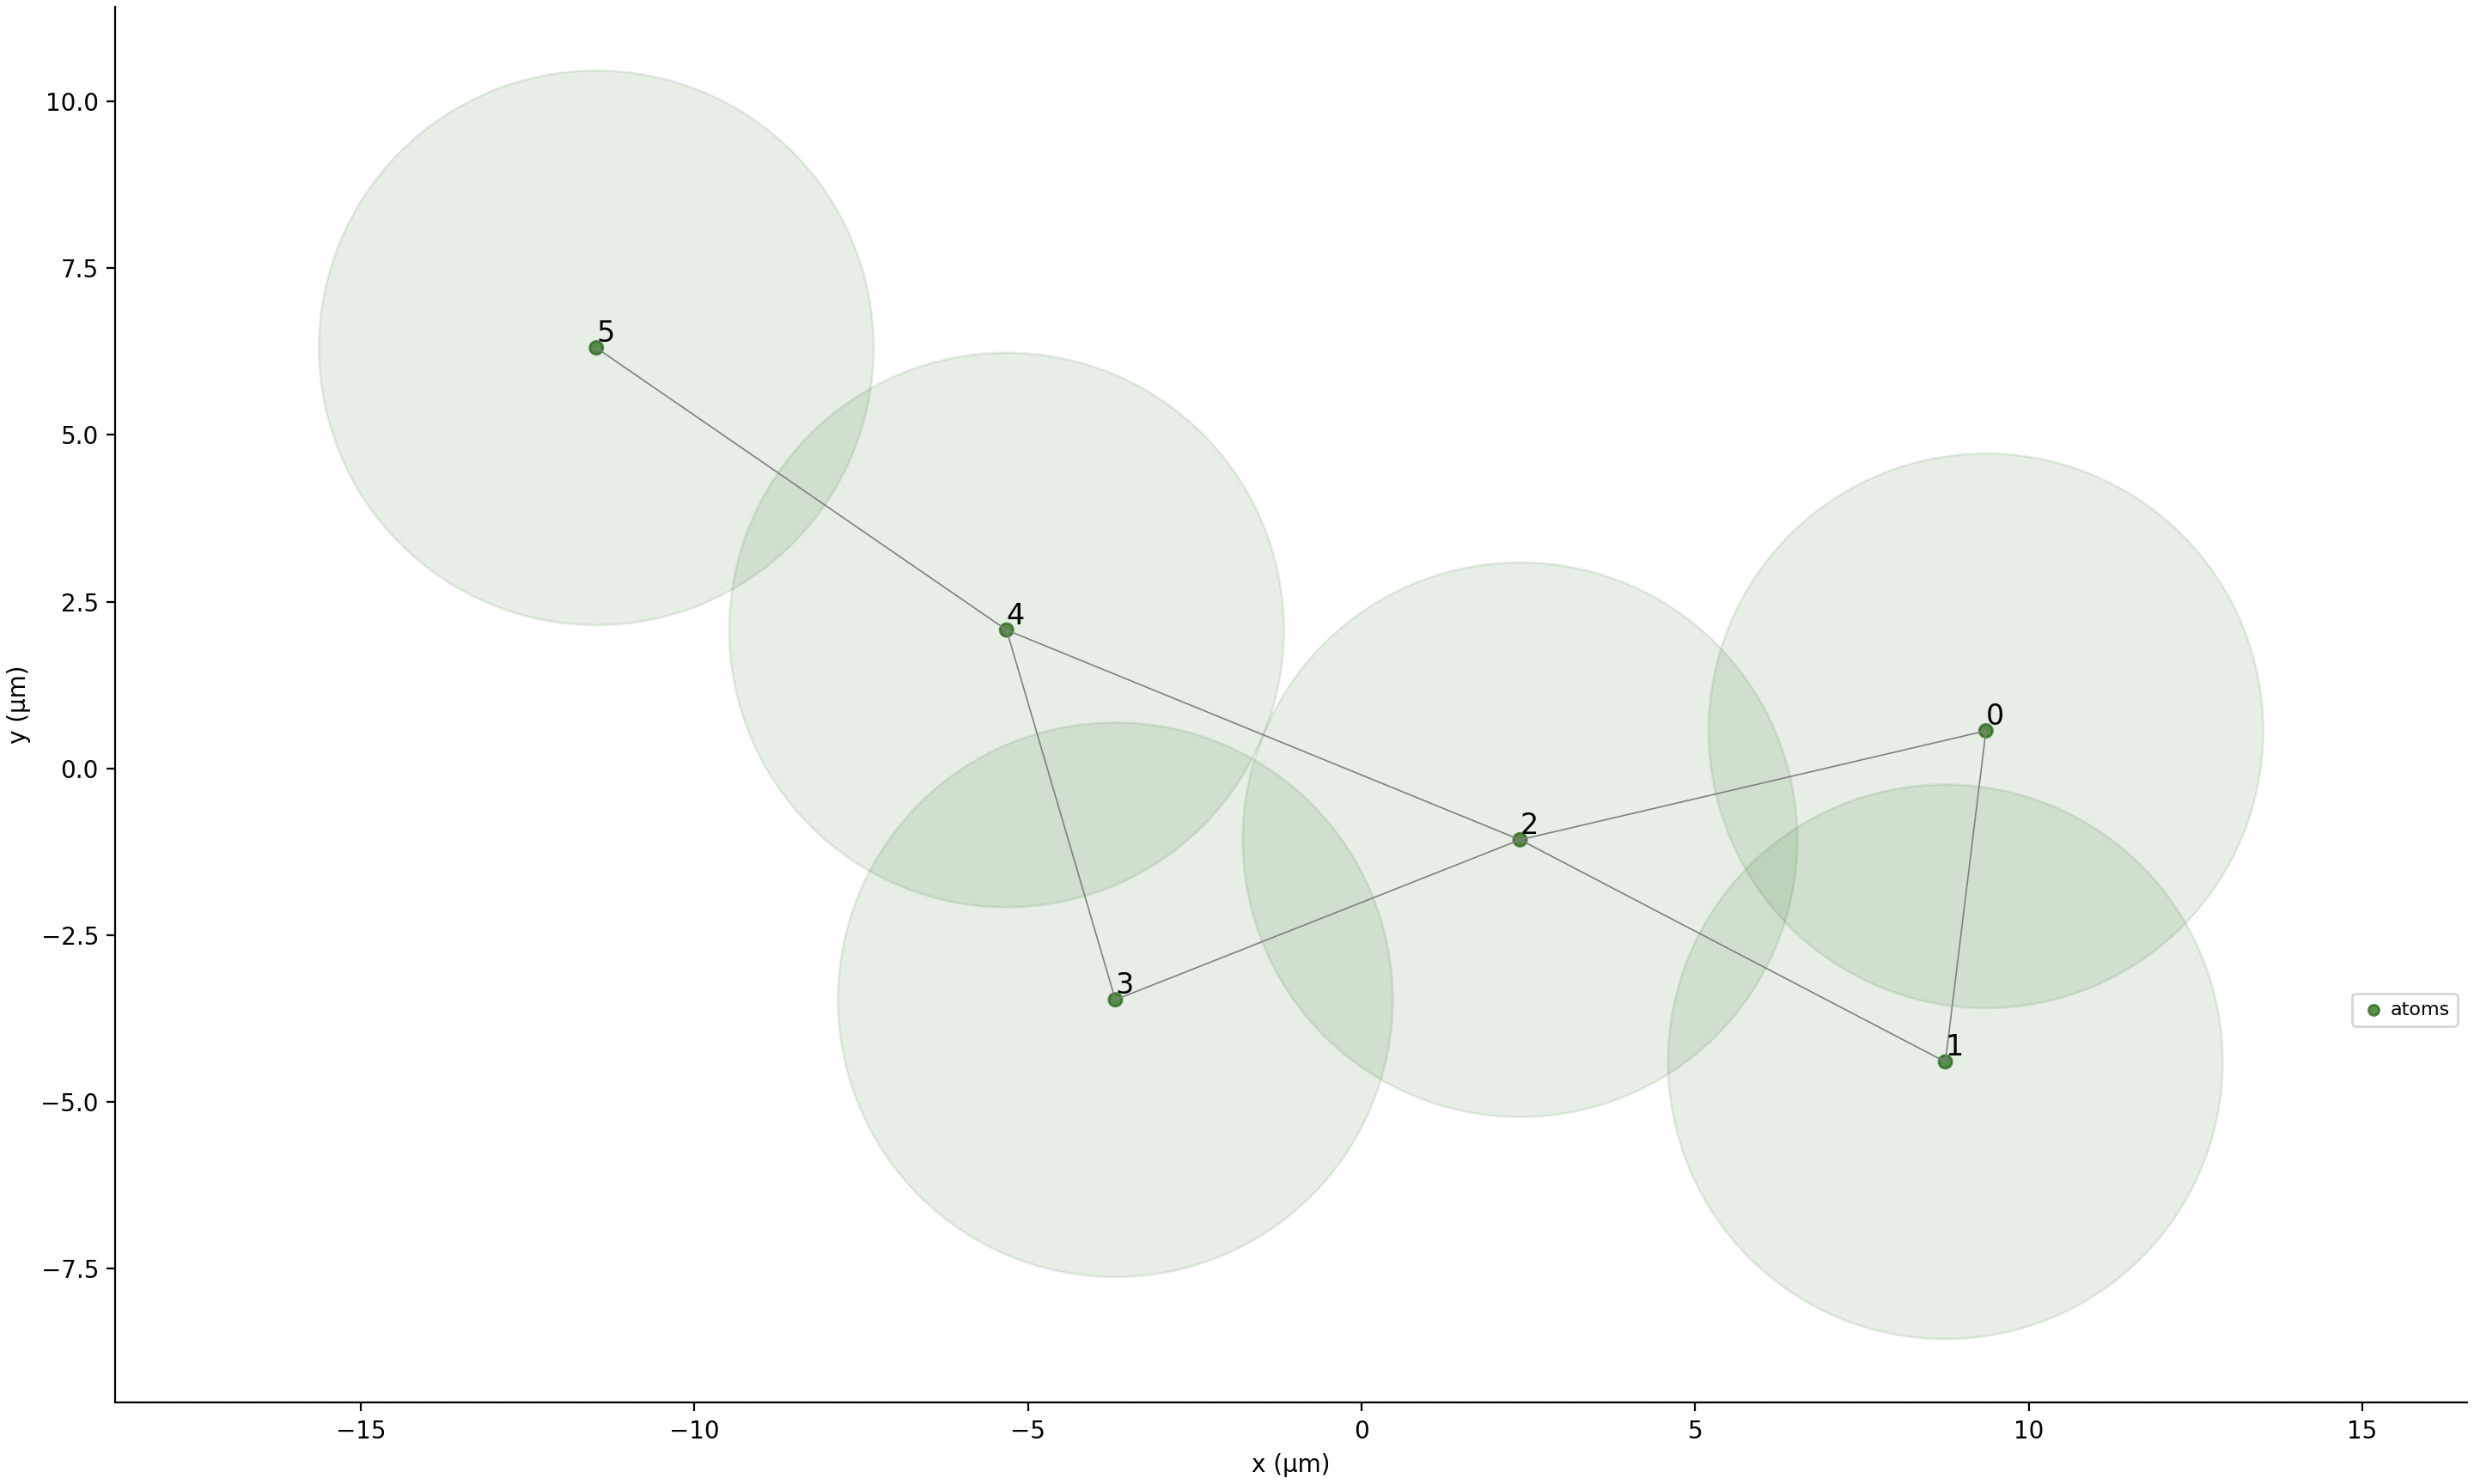
\includegraphics[width = 0.48\linewidth]{images/registre_exemple.png}
    \caption{Registre pour lequel les deux algorithmes quantiques seront testés sur un simulateur}
\end{figure}\label{graphtocompare}

Les performances des algorithmes seront comparées pour déterminer la méthode à employer pour résoudre de plus gros problèmes. En effet, les ressources pour tester les algorithmes sont limitées. Ainsi, une seule méthode se doit d'être explorée en détail pour avoir des résultats intéressants.

Pour les deux méthodes, le pulse \textit{Rise\_fall} et 1000 \textit{shots} seront utilisées.

\subsubsection{Détermination du pulse optimal}\label{pulse_opt}
Après avoir établi la méthode quantique la plus prometteuse, les pulses seront testés pour déterminer celui qui donne les meilleurs résultats. En effet les pulses suivants appliqués pendant $4 \mu s$ seront appliqués sur le registre de la figure \ref{graphtocompare}. 
\begin{itemize}
    \item "Rise\_sweep\_fall" : Ce pulse commence à 0, augmente jusqu'à la valeur de Omega spécifiée pendant le quart du temps, reste constant à cette valeur pendant la moitiée du temps et finalement redescend à 0 pour le dernier quart du temps. Les changements se font linéairement.

    \item "Pyramid" : Ce pulse commence à une valeur spécifiée de Omega moins un certain delta. Le pulse reste à cette valeur durant le quart du temps total. Le pulse fait ensuite un pulse de type "Rise\_fall" pendant la moitiée du temps total pour monter à Omega et redescendre à Omega - delta. Le pulse reste finalement constant pour le dernier quart du temps total à la valeur de Omega - delta.
    
    \item "Blackman" : Ce pulse est un pulse de forme normal avec comme aire total la valeur donnée de Omega.

    \item "Rise\_fall" : Ce pulse est simplement la partie "Rise\_fall" du pulse de type "Rise\_sweep\_fall". Le pulse commence à 0 et monte jusqu'à Omega pendant la moitié du temps. Le pulse redescend jusqu'à 0 pour la dernière moitié du temps. Les changements sont aussi linéaires. 

    \item "Waveform" : Ce pulse commence à 0, atteint Omega à la moitié du temps total et vaut de nouveau 0 à la fin du temps. La forme du changement suit une courbe qui ressemble le plus possible à une parabole.
\end{itemize}



La proportion de résultats valides du dictionnaire de retour sera évaluée. L'appareil \textit{AnalogDevice} sera utilisé pour cette prise de données.

\subsubsection{Évaluer la performance de l'algorithme de recombinaison de sous-graphe}\label{indep}
Ensuite, la performance de l'algorithme de recombinaison de graphe sera testée sur le graphe de 35 sommets de la figure \ref{35atoms} . Avec l'aide du puissant simulateur de Pascal permettant de rouler des algorithmes de calculs analogiques quantiques à environ 35 atomes, il sera possible d'appeler directement l'algorithme quantique ayant le mieux performé à l'étape précédente une seule fois pour le graphe. Ainsi, en exécutant l'algorithme classique n'ayant pas de limitations, l'algorithme quantique, nous allons pouvoir comparer la performance de ces algorithmes. Il sera aussi possible de voir si la recombinaison de sous-graphe donne une bonne approximation d'avoir rouler le graphe au complet dans un seul appel de MIS.


\begin{figure}[H]
    \centering
    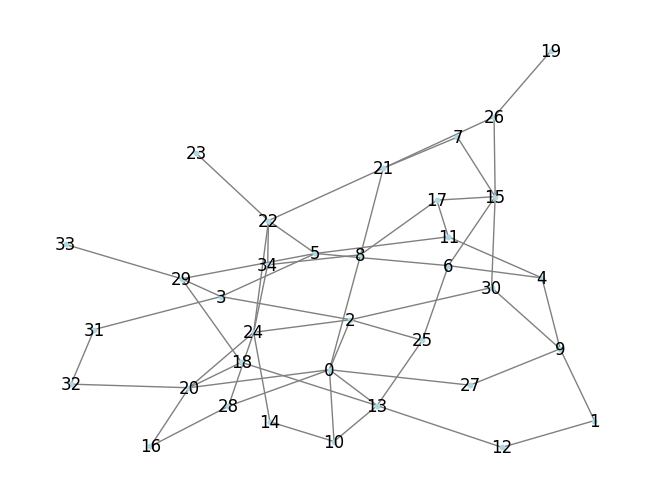
\includegraphics[width=0.49\linewidth]{images/35atomes.png}
    \caption{Graphe utilisé pour tester l'algorithme de recombinaison de graphe.}
    \label{35atoms}
\end{figure}

\subsection{Résoudre le problème de Récupex}
La réattribution des bacs plus efficace dans la ville se sépare en trois grandes étapes présentées dans les sous-sections suivantes.

\subsubsection{Tri de l'emplacement actuel des bacs}
La première étape consiste à retirer des bacs dans leur répartition actuelle. En effet, en utilisant un algorithme de MIS, des bacs seront enlevés. Le graphe sera construit comme suit:
\begin{itemize}
    \item Les bacs représenteront les sommets du graphe.
    \item Deux sommets du graphe sont reliés si les bacs en question sont à 1,5 km ou moins de distance. Par contre, cette arête est retiré si le volume moyen annuel de vêtement reçu de chacun des bacs impliqués est de plus de 27754 (ce nombre est la somme de la moyenne des volumes annuels receuilli par bav et leur l'écart-type). 
\end{itemize}
La solution maximisant le nombre de sommet est choisie. En cas d'galité, c'est celle générant le plus de volume moyen qui sera choisie. Notons $n$ le nombre de bacs retirés par le MIS.

\subsubsection{Raffiner la liste des endroits possibles}
Avec les données de l’ensemble indépendant maximal résultant, les commerces à un rayon de 1,5 km d'un bac seront retirés de la base de données des emplacements possibles de bacs. Les emplacements possibles sont discutés dans la théorie.

\subsubsection{Trouver les nouveaux endroits des bacs retirés}
Par la suite, un graphe sera créé avec la liste raffinée des endroits possibles pour mettre les bacs.
\begin{itemize}
    \item Les sommets seront les endroits possibles.
    \item Deux sommets seront reliés par une arrête si la distance entre leur endroit possible associé est moins de 2,8 km. Par la suite, un algorithme de MIS sera utilisé pour obtenir la nouvelle distribution des bacs.
\end{itemize}

Le choix des distances est arbitraire. Le choix a été fait dans le but d'obtenir une nouvelle distribution d'environ 60 bacs.
Cette méthodologie sera exécutée pour la méthode classique où chacun des MIS sera exécuté 100 fois pour obtenir le résultat approprié selon l'étape (décrit plus haut).
Elle sera aussi exécutée avec la méthode trouvant des MIS en divisant en sous-graphes où chacun des sous-mis est exécuté 100 fois avec le pulse  "Rise-Fall" de $4000 \mu s$ avec la méthode quantique adiabatique. La première étape sera faite avec des sous-graphe d'au plus 10 atomes et la troisième avec au plus 7 atomes. Ces paramètres ont été choisis après plusieurs tests parc qu'ils donnaient la meilleure distribution. De plus, le \textit{device DigitalAnalogDevice} a été utilisé pour traiter de plus gros graphe plus facilement.



\section{Résultats}
\subsection{Comparaison du QAA et QAOA}
\begin{figure}[H]
    \centering
    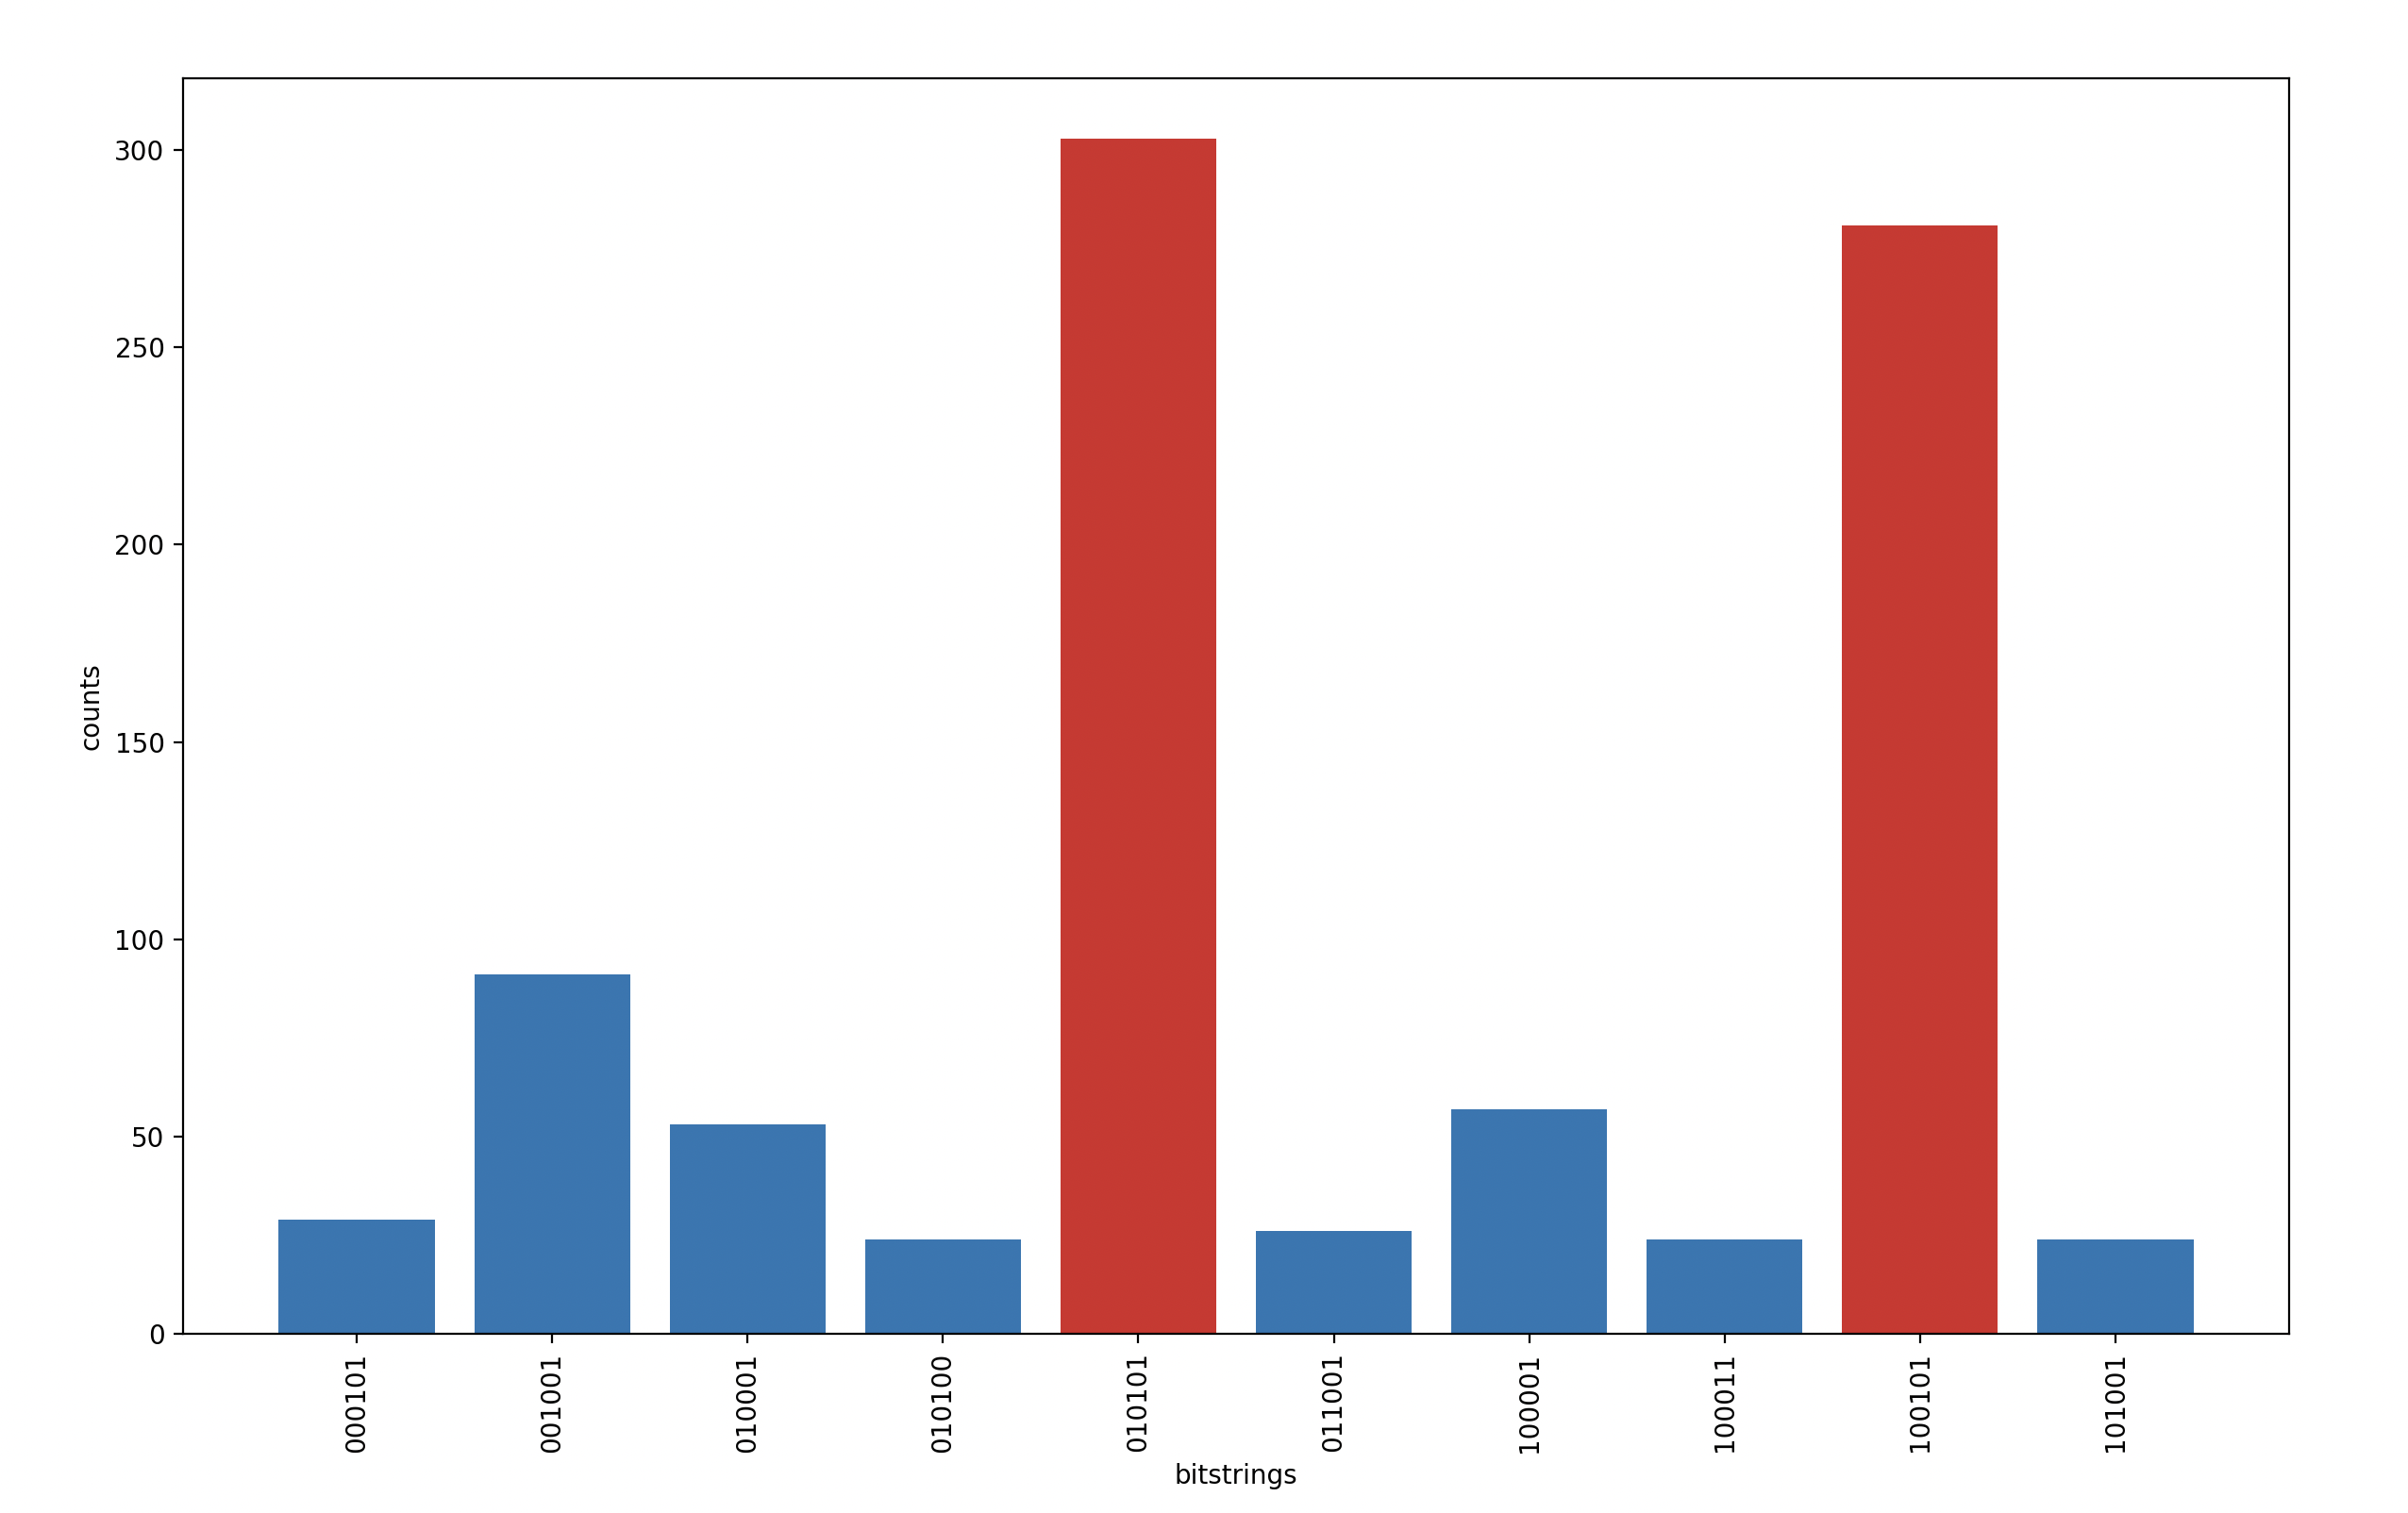
\includegraphics[width = 0.50\linewidth]{images/histo_qaa_exemple.png}
    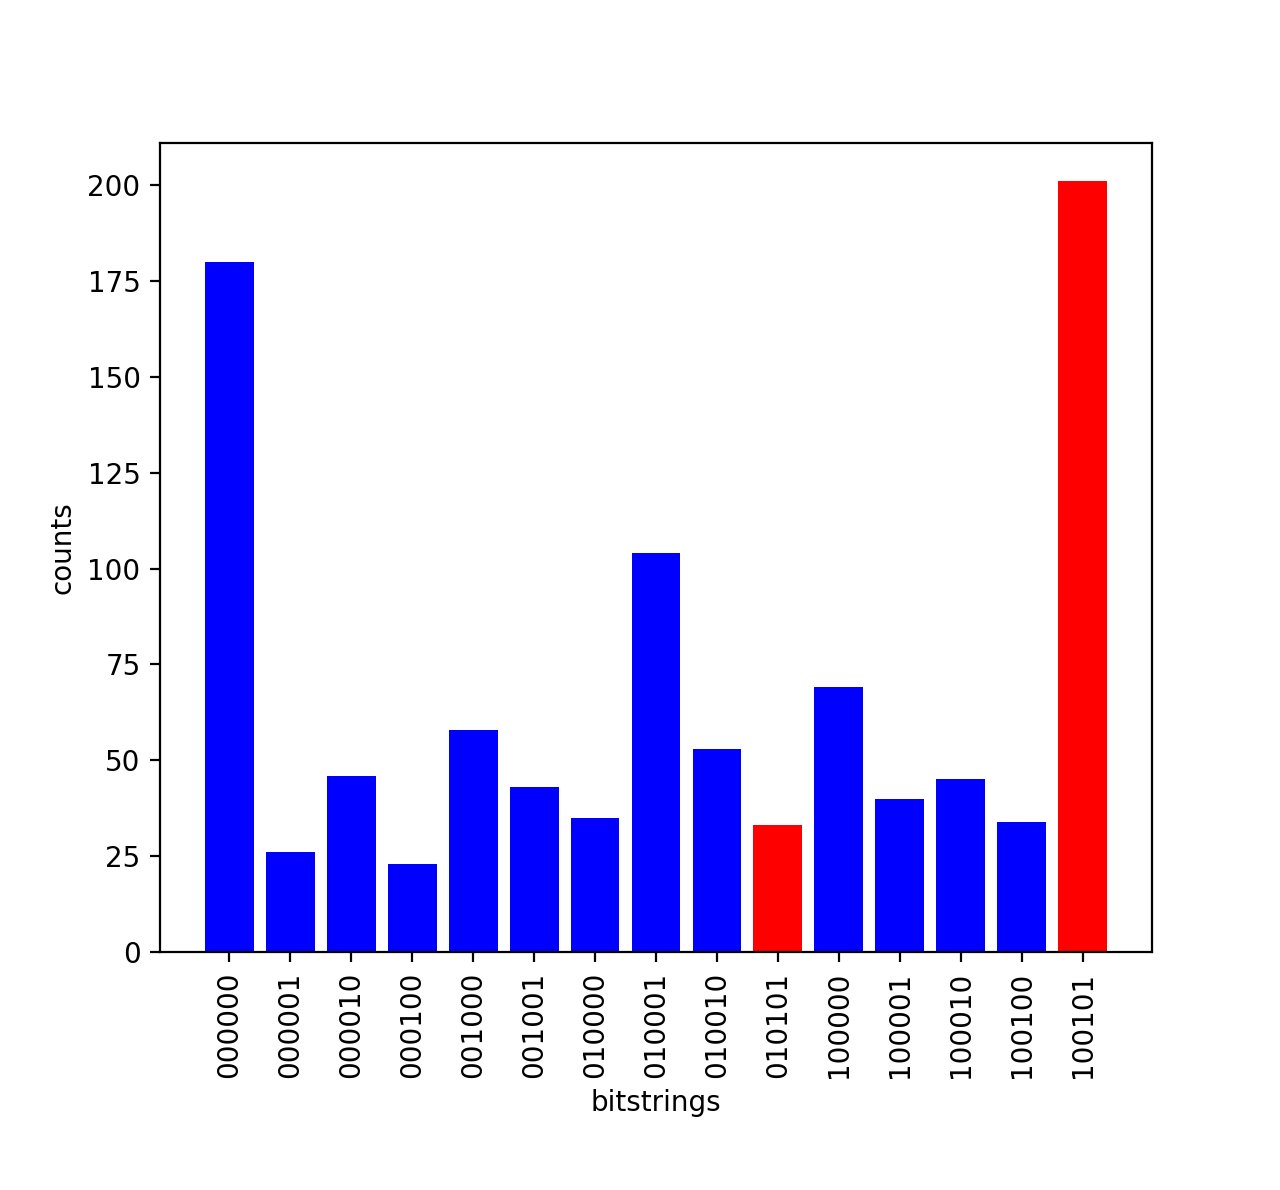
\includegraphics[width=0.45\linewidth]{images/qaoa_res.png}
    \caption{Histogrammes retournés, à gauche par l'algorthme adiabatique et à droite par le QAOA pour le MIS du graphe de la figure \ref{graph_exemple}}
    \label{qaoavsqaa}
\end{figure}

\subsection{Détermination du pulse optimal}
\begin{figure}[H]
    \centering
    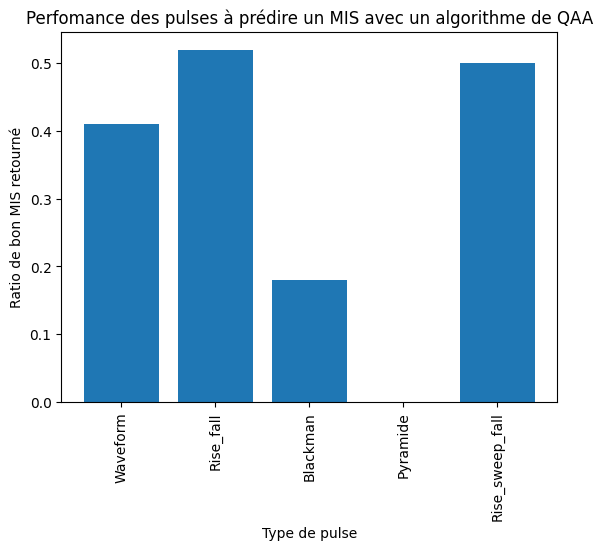
\includegraphics[width=0.49\linewidth]{images/pusle_comp.png}
    \caption{Comparaison de la performance des pulses sur le graphe de la figure \ref{MIS_exemple} avec la méthode de QAA. L'appareil \textit{Analogdevice} a été utilisé pour les pulses durant 4000$\mu s$.}
    \label{pulse_comp}
\end{figure}

\subsection{Analyse de l'algorithme de recombinaison de graphe}
\begin{figure}[H]
    \centering
    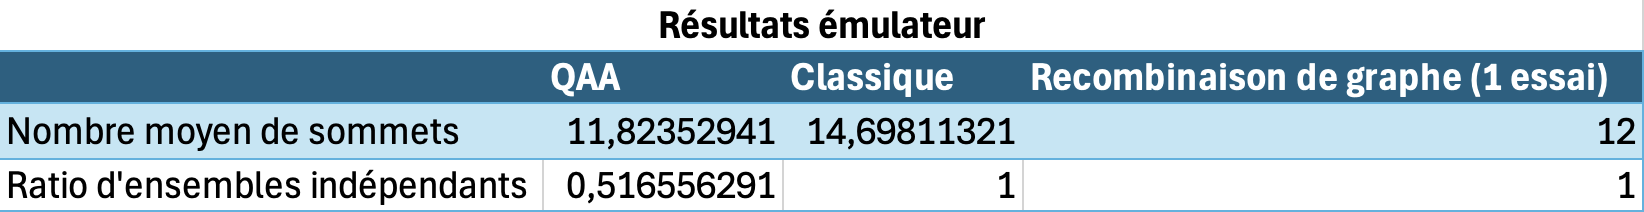
\includegraphics[width=0.70\linewidth]{images/table_emul.png}
    \caption{Table des résultats d'un graphe à 35 atomes roulé sur l'émalateur de Pascal. Pour les données présentées, seule les réponse données plus d'une fois par l'ordinateur sont considérées.}
    \label{emul_stats}
\end{figure}

\subsection{Solution au problème de Récupex}
\begin{figure}[H]
    \centering
    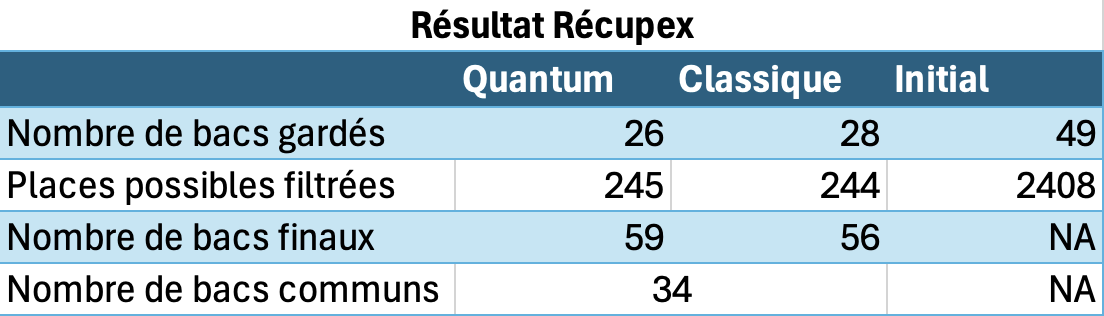
\includegraphics[width=0.49\linewidth]{images/recupex_solver.png}
    \caption{Statistiques de placement des bacs pour le problème de Recupex. La méthode quantique choisie est le QAA.}
    \label{recupex_stats}
\end{figure}


\begin{figure}[H]
    \centering
    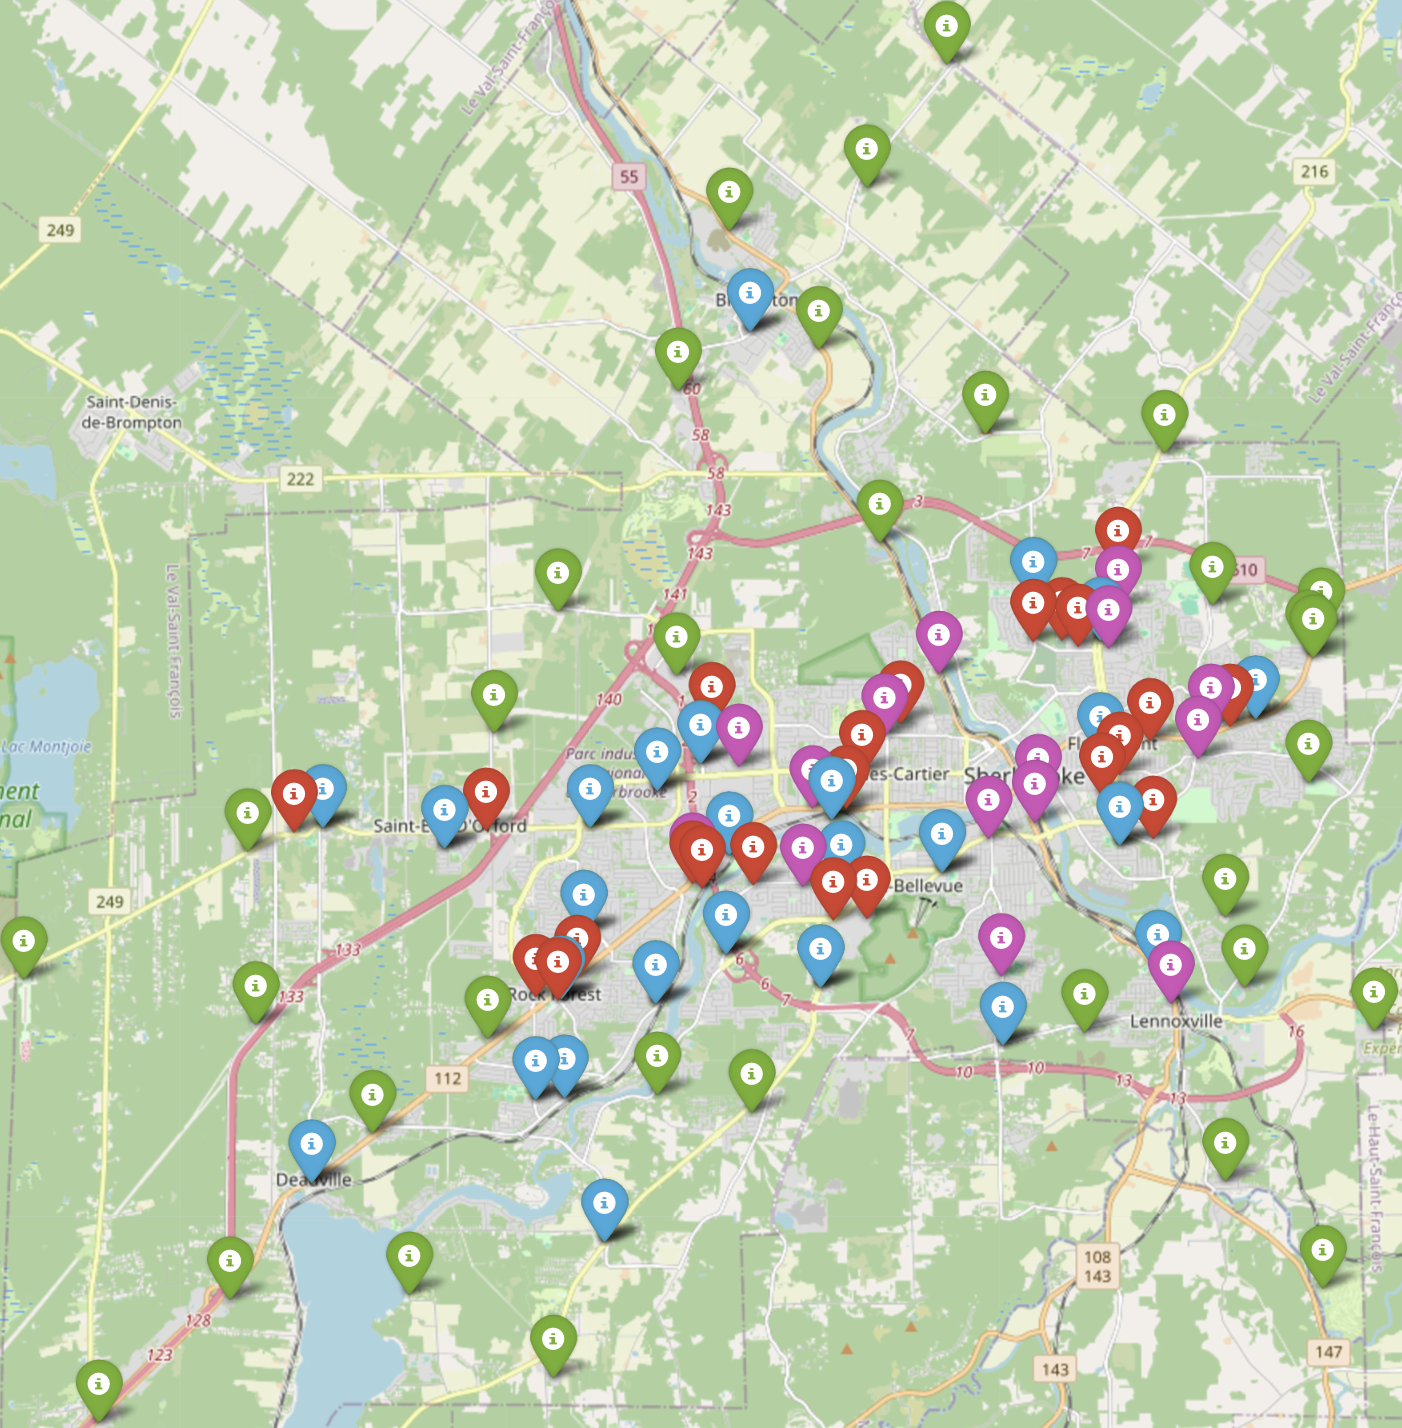
\includegraphics[width=0.49\linewidth]{images/total_quantum.png}
    \caption{Carte des cloches après l'usage de notre algorithme quantique de QAA (les points \textcolor{Mulberry}{violets} représentent les bacs d'Estrie-Aide, les points \textcolor{LimeGreen}{verts} représentent les bacs ajoutés, les points \textcolor{BrickRed}{rouges} représentent les bacs enlevés et les points \textcolor{CornflowerBlue}{bleus} représentent les bacs conservés).
}
    \label{total}
\end{figure}

\begin{figure}[H]
    \centering
    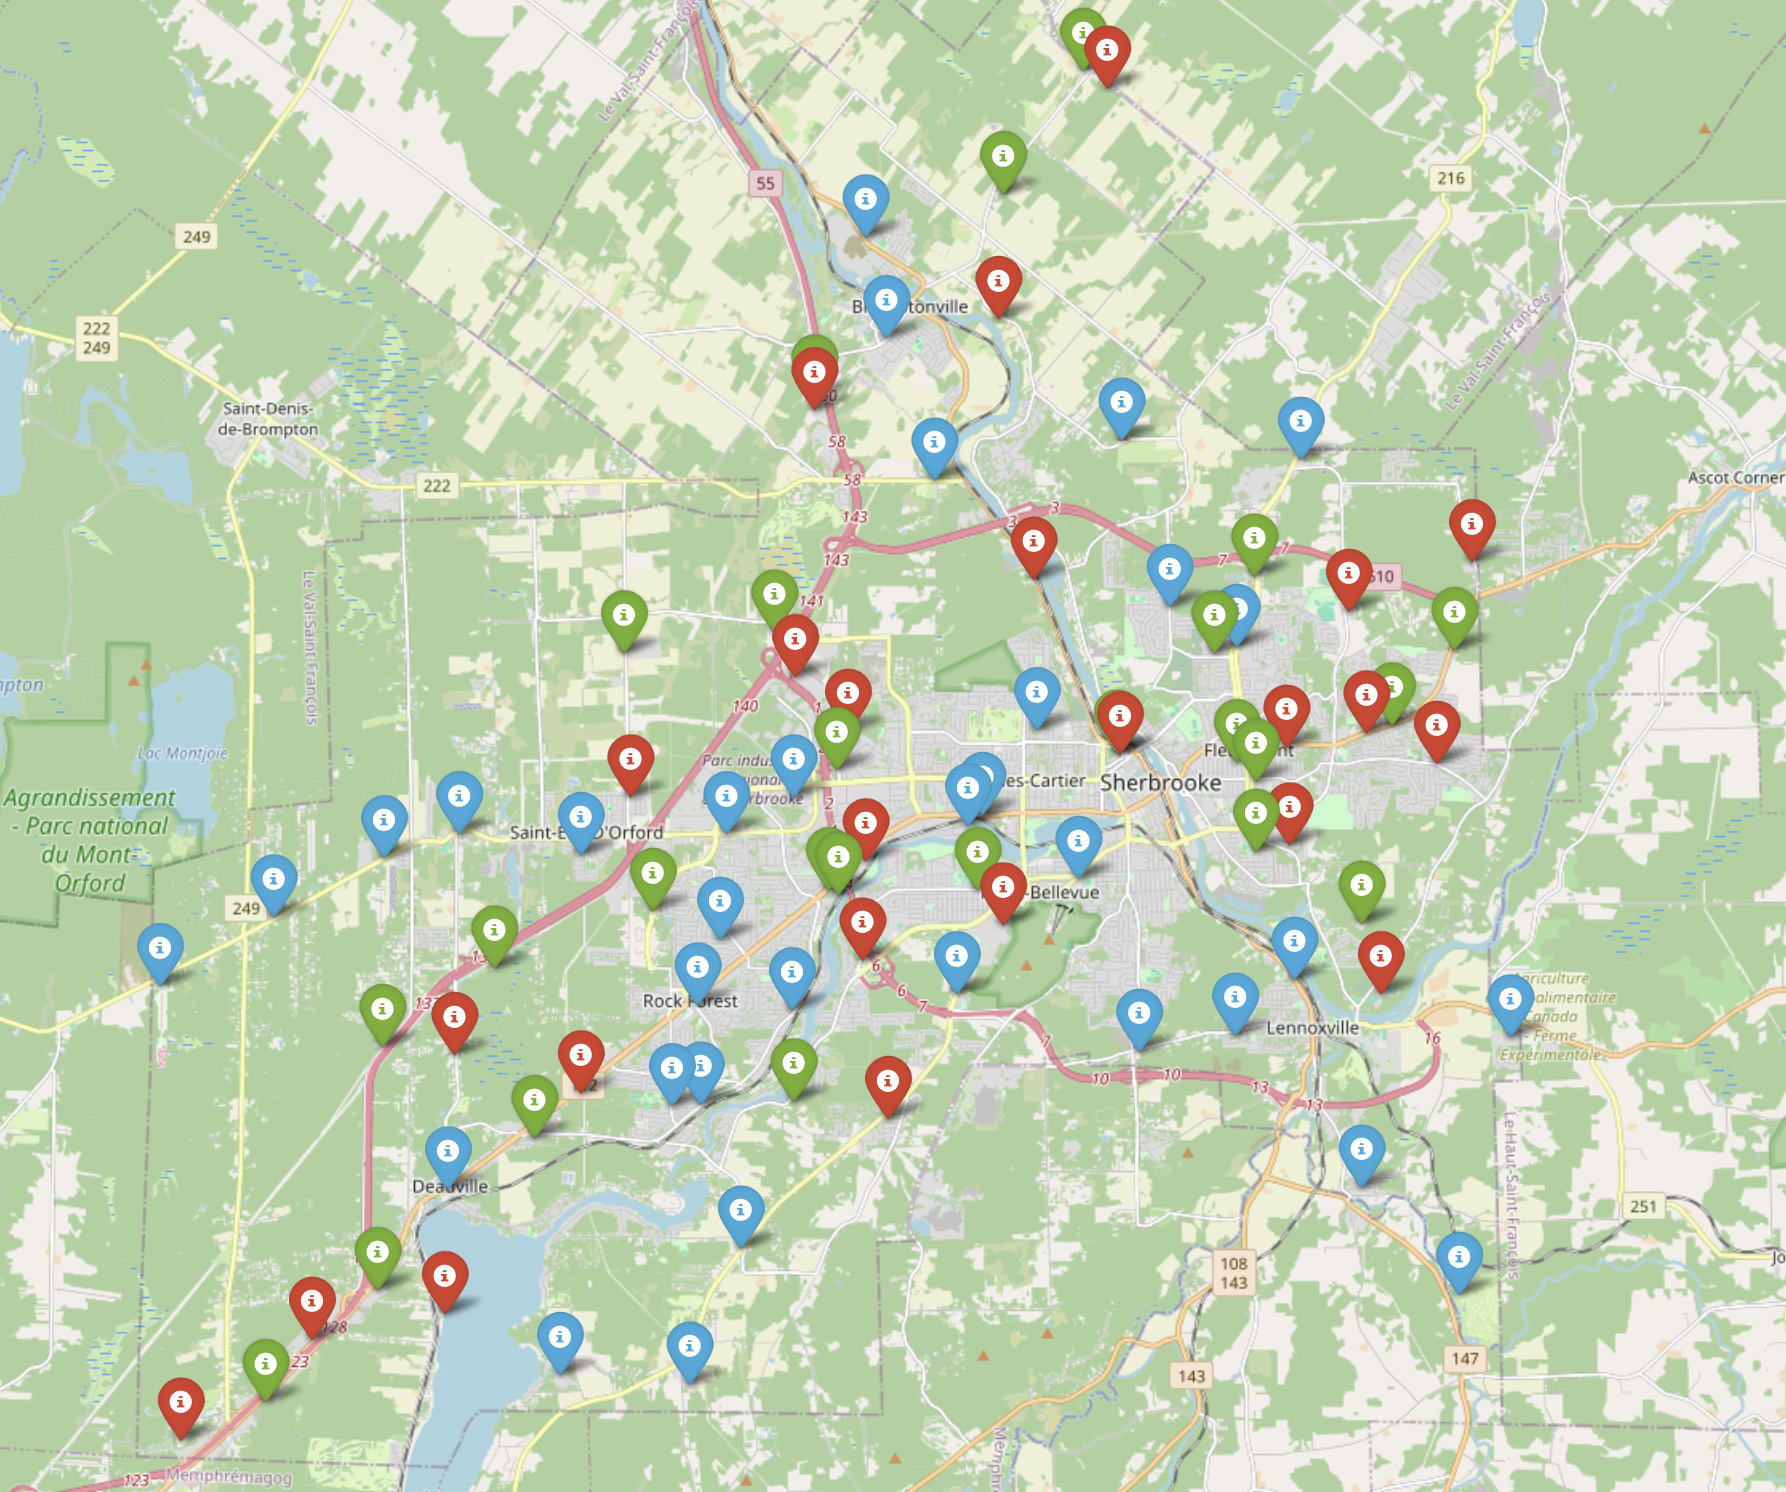
\includegraphics[width=0.49\linewidth]{images/both_distributions.png}
    \caption{Carte de la comparaison des emplacements choisis par la méthode classique et quantique (les points \textcolor{LimeGreen}{verts} représentent les bacs seulement dans la distribution des bacs obtenus par la méthode quantique, les points \textcolor{BrickRed}{rouges} représentent les bacs seulement dans la distribution des bacs obtenus par la méthode classique et les points \textcolor{CornflowerBlue}{bleus} représentent les bacs observés dans les deux distributions).
}
    \label{bothdist}
\end{figure}

\section{Discussion}

\subsection{Algorithme d'optimisation approximative quantique}

 On peut observer que les bitstrings correspondant aux solutions optimales sont présents, mais pas avec la fréquence la plus élevée pour la méthode de QAOA (l'histogramme de droite de la figure \ref{qaoavsqaa}). Cela s'explique par la profondeur limitée du circuit QAOA, qui empêche l'algorithme de converger pleinement vers les solutions optimales. De plus, d'autres bitstrings non optimaux apparaissent avec des fréquences significatives, ce qui reflète une exploration plus variée de l'espace des solutions.
En comparaison, les résultats obtenus avec la méthode QAA (\textit{Quantum Adiabatic Algorithm}) (l'histogramme de gauche de la figure \ref{qaoavsqaa}) montrent une concentration beaucoup plus marquée sur les solutions optimales, ce qui est représentée l'histogramme correspondant. Cela prouve que, bien que le QAOA permette une exploration plus large, il est moins déterministe que le QAA.




Ainsi, bien que cette méthode soit moins limitée en termes de coût, elle nécessite une profondeur de circuit importante pour obtenir des résultats satisfaisants, ce qui rend l'optimisation plus complexe. Une conclusion similaire a été observée dans le tutoriel de Pasqal (\textbf{citer ici}) avec un problème QUBO (\textit{Quadratic Unconstrained Binary Optimization}).

En conclusion, bien que l'algorithme d'optimisation approximative quantique ne soit pas la méthode optimale pour un problème comme le MIS, il constitue néanmoins une approche alternative intéressante à explorer pour d'autres types de problèmes, où il pourrait offrir de meilleures performances.

Pour les prochains résultats, l'algorithme de QAA a été utilisé dû à ces résultats.

\subsection{Analyse du pulse}
La figure \ref{pulse_comp} indique que certains pulses fonctionne mieux avec le QAA (méthode quantique préférable). Il est normal de remarquer que le pulse pyramide performe moins bien, puisque sa valeur d'omega est constante à une valeur plus basse que l'omega maximal pendant la moitié du temps total. Aussi, le pulse blackman n'est pas efficace pour notre projet, puisque nous n'avons pas de contrôle sur la valeur d'omega maximum qui détermine le rayon de blocage. L'aire du pulse n'est pas très importante pour notre projet. Les trois autres pulses sont comparables, puisqu'ils respectent toutes les conditions de pulse nécessaires pour trouver l'ensemble maximal indépendant. Ils atteingent tous la fréquence de Rabi au milieu du temps total afin de déterminer le rayon de blocage.
On trouve finalement que entre les pulses \textit{Rise\_fall, Rise\_sweep\_fall, Waveform}, le pulse \textit{Rise\_fall} semble obtenir de meilleur résultats dans le contexte de notre projet.

L'appareil \textit{AnalogDevice} a été employés puisqu'il présentait des meilleurs résultats pour des plus petits graphes. En effet, pour le graphe en exemple, en utilisant l'appareil \textit{DigitalAnalogDevice}, des résultats très faibles étaient présentés. Par contre, la même tendance entre les pulse était présente. En contre partie, pour rouler des graphes plus grands, l'appareil \textit{DigitalAnalogDevice} sera utilisé.

Ainsi, pour le reste des résultats le pulse \textit{Rise\_fall} a été utilisé avec un temps de $4000 \mu s$.

\subsection{Performance pour la résolution du problème de Récupex}
Pour résoudre le problème de Recupex, la méthode QAA et classique ont été utilisés. En effet, comme mentionné plus tôt, la méthode de "QAOA" ne donnait pas des résultats satisfaisants sur des petits graphes. 

Il est possible de remarquer que la méthode classique donne des résultats beaucoup plus rapidement que le QAA. Effectivement, le fait de rouler plusieurs simulations quantiques prend beaucoup de temps. Même si sur un ordinateur quantique le temps de calcul sera moindre, le fait de préparer le système d'atome neutre 100 fois par sous-graphe prend aussi beaucoup de temps. Il y a donc un avantage d'utiliser la méthode classique lorsque plus d'emplacements possibles seront considérés. De plus, la figure \ref{bothdist} indique que les deux méthodes font tout de même une bonne distribution des bacs en choisissant une majorité de mêmes bacs. Effectivement, la tableau de la figure \ref{recupex_stats} indique que plus de la moitié des  bacs choisis sont communs dans les deux méthodes. Cela indique que le premier ensemble indépendant trouvé maximisant le volume est semblable pour les deux méthodes.  Par la suite, à l'ajout des nouveaux bacs, quelques différences sont notées par la grandeur du réseau d'emplacement possible et leur interconnexion. Dans les deux cas, les deux méthodes ont réussi à bien couvrir la surface de Sherbrooke en entier. En effet, la couverture du territoire comparé à la répartition originale est bien meilleure et présentée en annexe à la figure \ref{new_dist}. Les deux méthodes ont environ le même nombre de bacs. Il n'est pas surprenant d'observer que la méthode quantique retourne une distribution avec plus de bacs puisque cette méthode retourne moins facilement des ensemble indépendants (discutés à la section \ref{Mi}). Ainsi, la méthode quantique place quelques bacs trop près l'un des autres. En général, la solution générale quantique approxime bien la classique.



Par contre, il est important de noter que le résultat proposé par la version quantique est limité à des sous-graphes traités par la méthode quantique à 10 sommets pour la première partie et la dernière partie à 7 sommets. En faisant cela, les MIS résultant des sous-graphes ne sont pas autant significatifs que souhaité puisque la majorité des calculs se fait par la recombinaison de plusieurs petits sous-graphes ayant un MIS trivial qui ne nécessiterait pas le quantique. Des avenues pour résoudre ce problème seront présentées dans la prochaine section. Il est important aussi de prendre en compte les ressources nécessaires afin d'obtenir la solution quantique. Disons qu'hypotétiquement, une entreprise donne accès à un ordinateur quantique à atome neutre au coût d'une cent par calcul. Puisque l'algorithme est probabibiliste et que nous devons effectuer plusieurs algorithmes sur différents graphe, le calcul devient rapidement dispendieux. En effet, la détermination d'un seul ensemble indépendant maximal coûte environ 100 calculs, c'est-à-dire 1\$. Supposons maintenant qu'on souhaite plus de précision et qu'on décide d'effectuer 1000 calculs au lieu de 100. On arrive donc à 10\$ par ensemble indépendant maximal. Cependant, notre algorithme nécessite plusieurs ensemble indépendants maximals (on approxime le nombre à 40). Ainsi, le coût total pour avoir une bonne réponse sans revérification serait environ de $40\cdot10\$ = 400\$$. 


\section{Pistes d'amélioration}

On peut espérer que, dans le futur, l'ordinateur quantique à atome neutre continue d'évoluer et nous permette d'utiliser un plus grand registre contenant plus d'atomes \cite{noauthor_pasqal_nodate}. De cette façon, nous n'aurions plus besoin d'approximer le graphe total en plusieurs sous-graphes et obtenir seulement un ensemble indépendant maximal approximatif à cause de la recombinaison. Nous trouverions plutôt les ensembles indépendants maximals et nous pourrions obtenir une meilleure solution plus simplement. Si on suit la feuille de route de Pasqal, le problème devrait être soluble sans avoir à couper le graphe dans les prochaines années \cite{noauthor_our_nodate}. De plus, l'utilisation d'un vrai ordinateur quantique fiable (sans trop de bruit) pourra potentiellement donner des meilleurs résultats pour des grands graphes.

Aussi, même si le QAOA ne performait pas autant bien sur des plus petits graphes, il aurait été intéressant d'explorer son utilisation sur de plus grosses instances. Peut-être que cette méthode aurait été plus facile à simuler ou offre de meilleurs résultats pour de gros systèmes?

D'autres méthodes de création d'un registre devraient être explorées. C'est principalement le registre qui limite l'algorithme d'ensemble indépendant maximal du QAA puisqu'il est difficile de mettre en registre n'importe quel graphe en général. Une méthode intéressante de création de registre a explorer est le "king's lattice" \cite{kim_quantum_2023}.

Aussi, une fonction de coût pourrait être utilisée afin de déterminer si le registre construit représente bien le graph. Une méthode d'optimisation afin de créer un meilleur registre pourrait être exploré.


\section{Conclusion}
En conclusion, l'algorithme quantique présente peu d’avantages lorsqu'il est comparé à la méthode classique. En effet, les limitations actuelles des ressources font en sorte que seulement des petits systèmes peuvent être traités avec précision. De ce fait, seulement des réponses approximatives à des problèmes de plus grande taille. Alors, plusieurs répétitions de l'algorithme classique sont suggérées pour résoudre des problèmes d'ensemble indépendant maximal. 

Aussi, une solution au problème de Recupex a été fournie. Peu de différences entre les deux méthodes ont été observées. Par contre, la méthode quantique a tendance à moins respecter les contraintes en plus de prendre plus de temps à exécuter au simulateur. Si l'algorithme était roulé sur un vrai ordinateur quantique, le coût serait aussi plus élevé.

Ainsi, avec les infrastructures quantiques actuelles ne permettent pas d'observer un réel avantage d'utiliser l'information quantique pour trouver des ensembles indépendants maximaux. En effet, l'utilisation de simulateurs limités en nombres d'atomes ne donne pas de meilleurs résultats. Il serait intéressant de tester le plus grand problème sur une technologie mature. En effet, sans avoir besoin de subdiviser les graphes, de meilleurs résultats pourraient être observés. Aussi d'autres pistes d'optimisation de pulse et de registre ont été proposées.

En bref, la méthode classique pour déterminer un MIS est encore plus puissante que la méthode quantique tant que les infrastructures quantiques ne sont pas plus développées, il est difficile de justifier leur utilisation et leur performance sur des problèmes de taille substantielle.

\section{Références}
\printbibliography[heading=none]

\section{Annexe}

\begin{figure}[H]
    \centering
    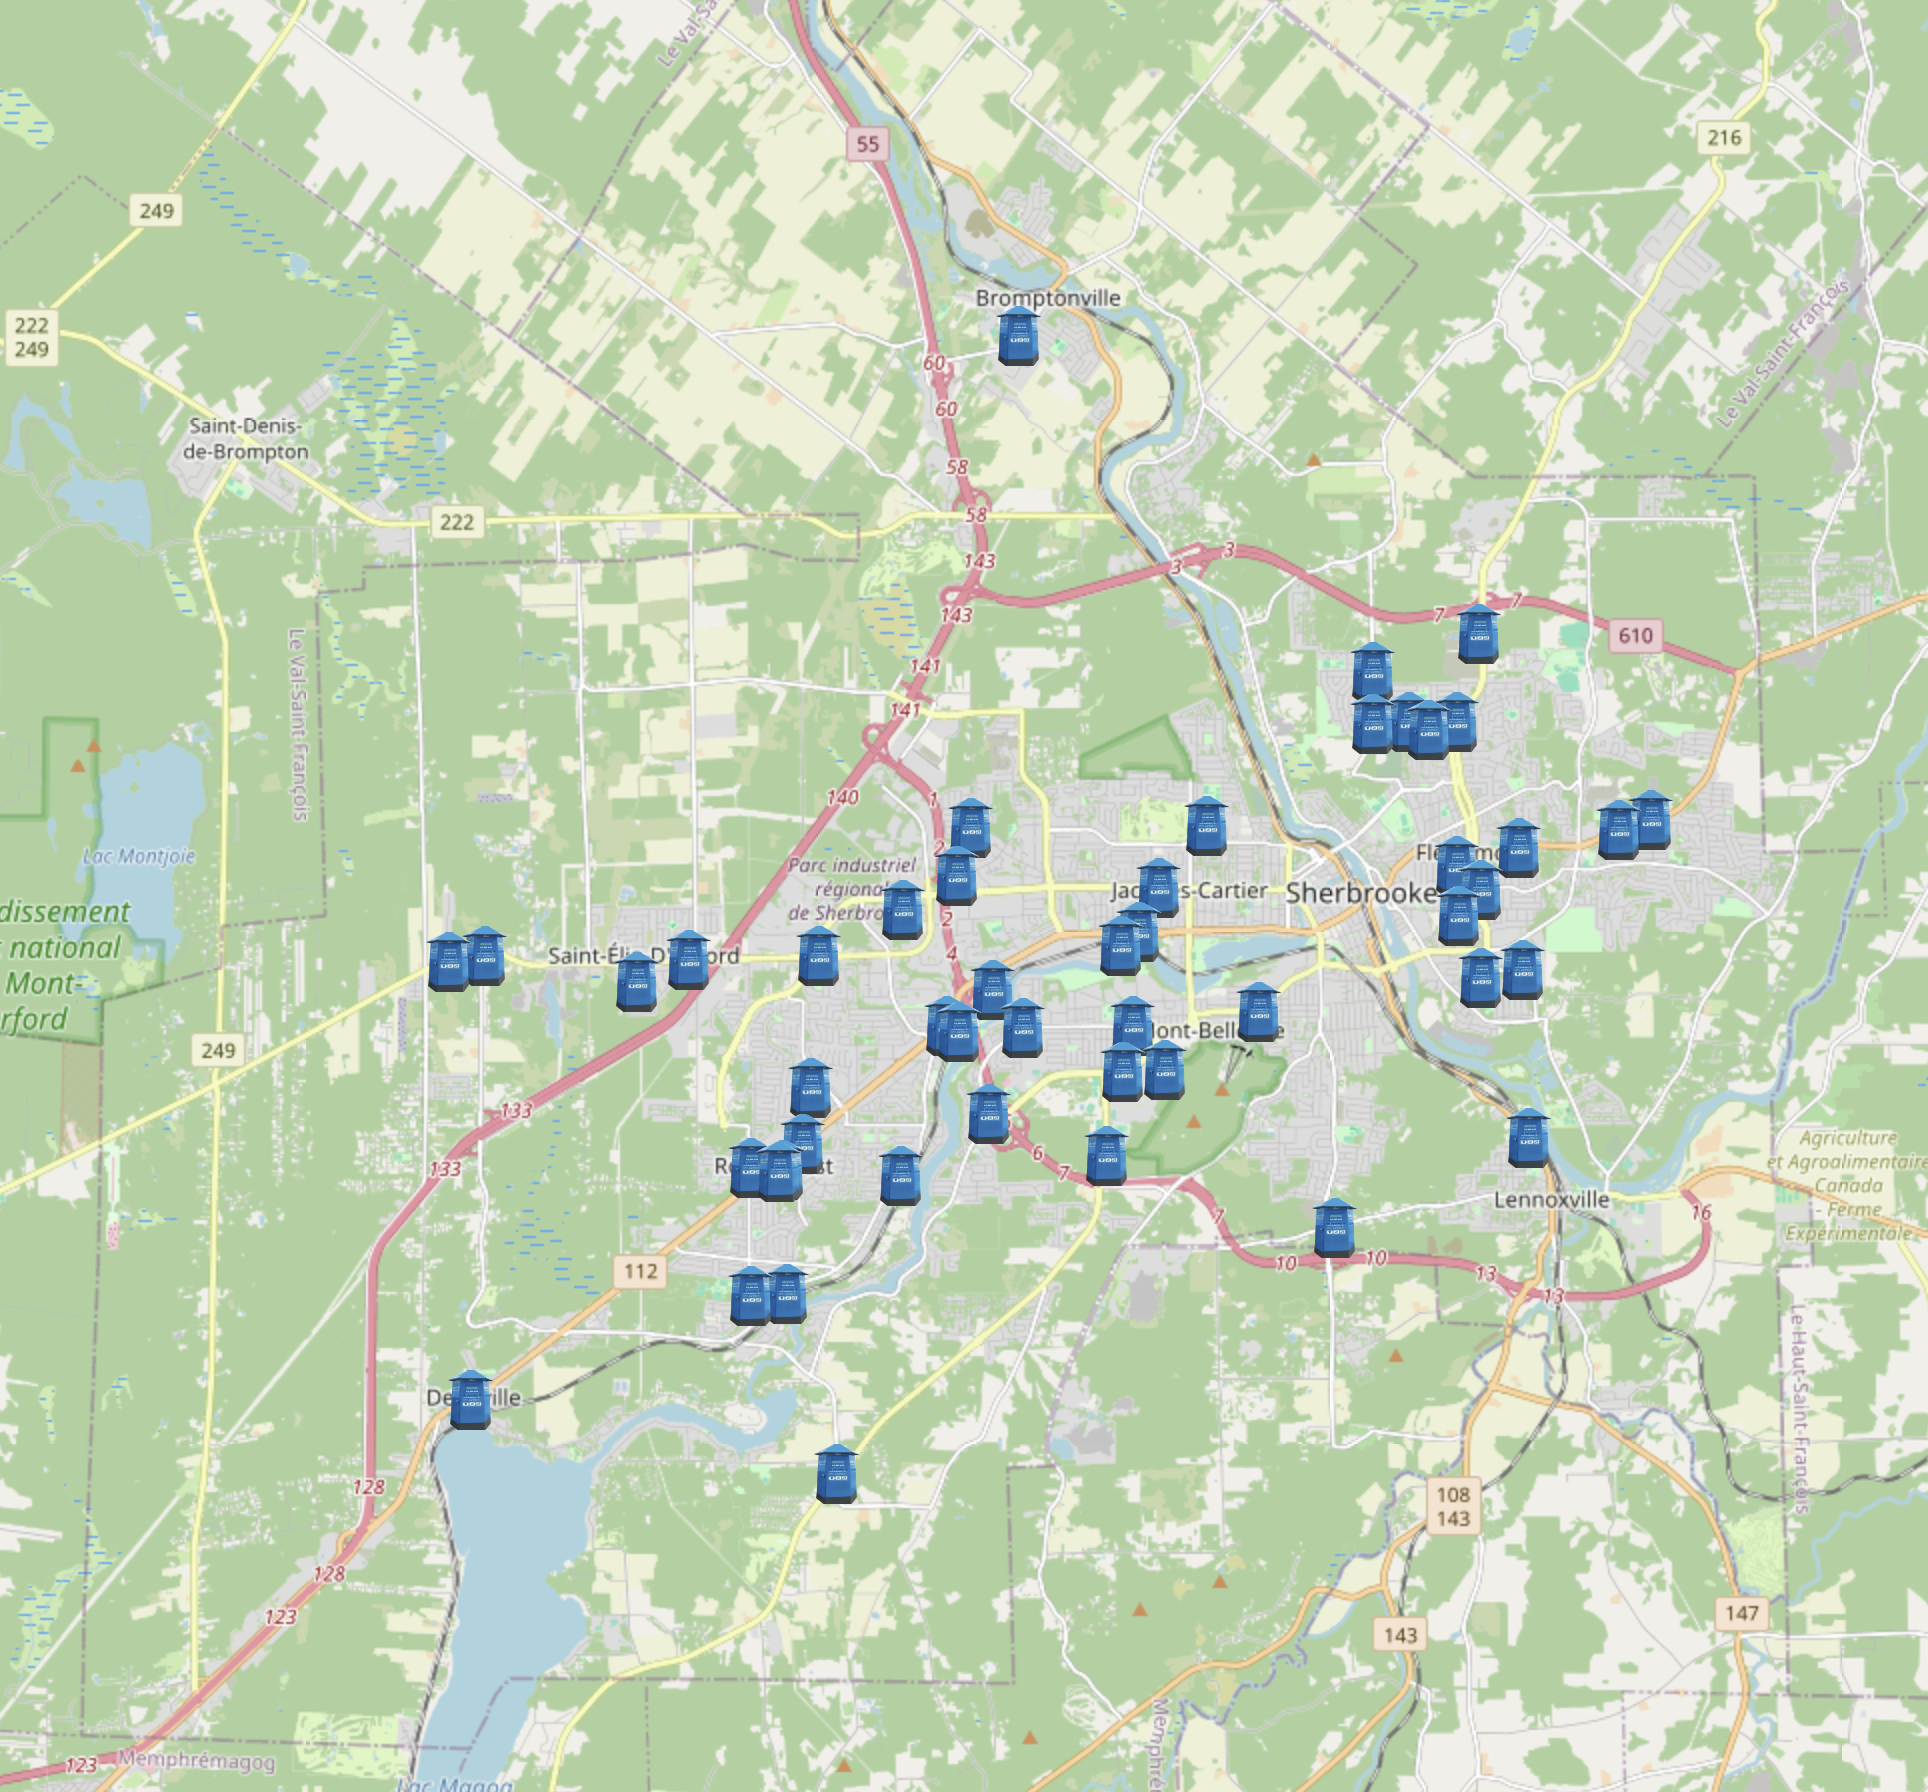
\includegraphics[width=0.33\linewidth]{images/original.png}
    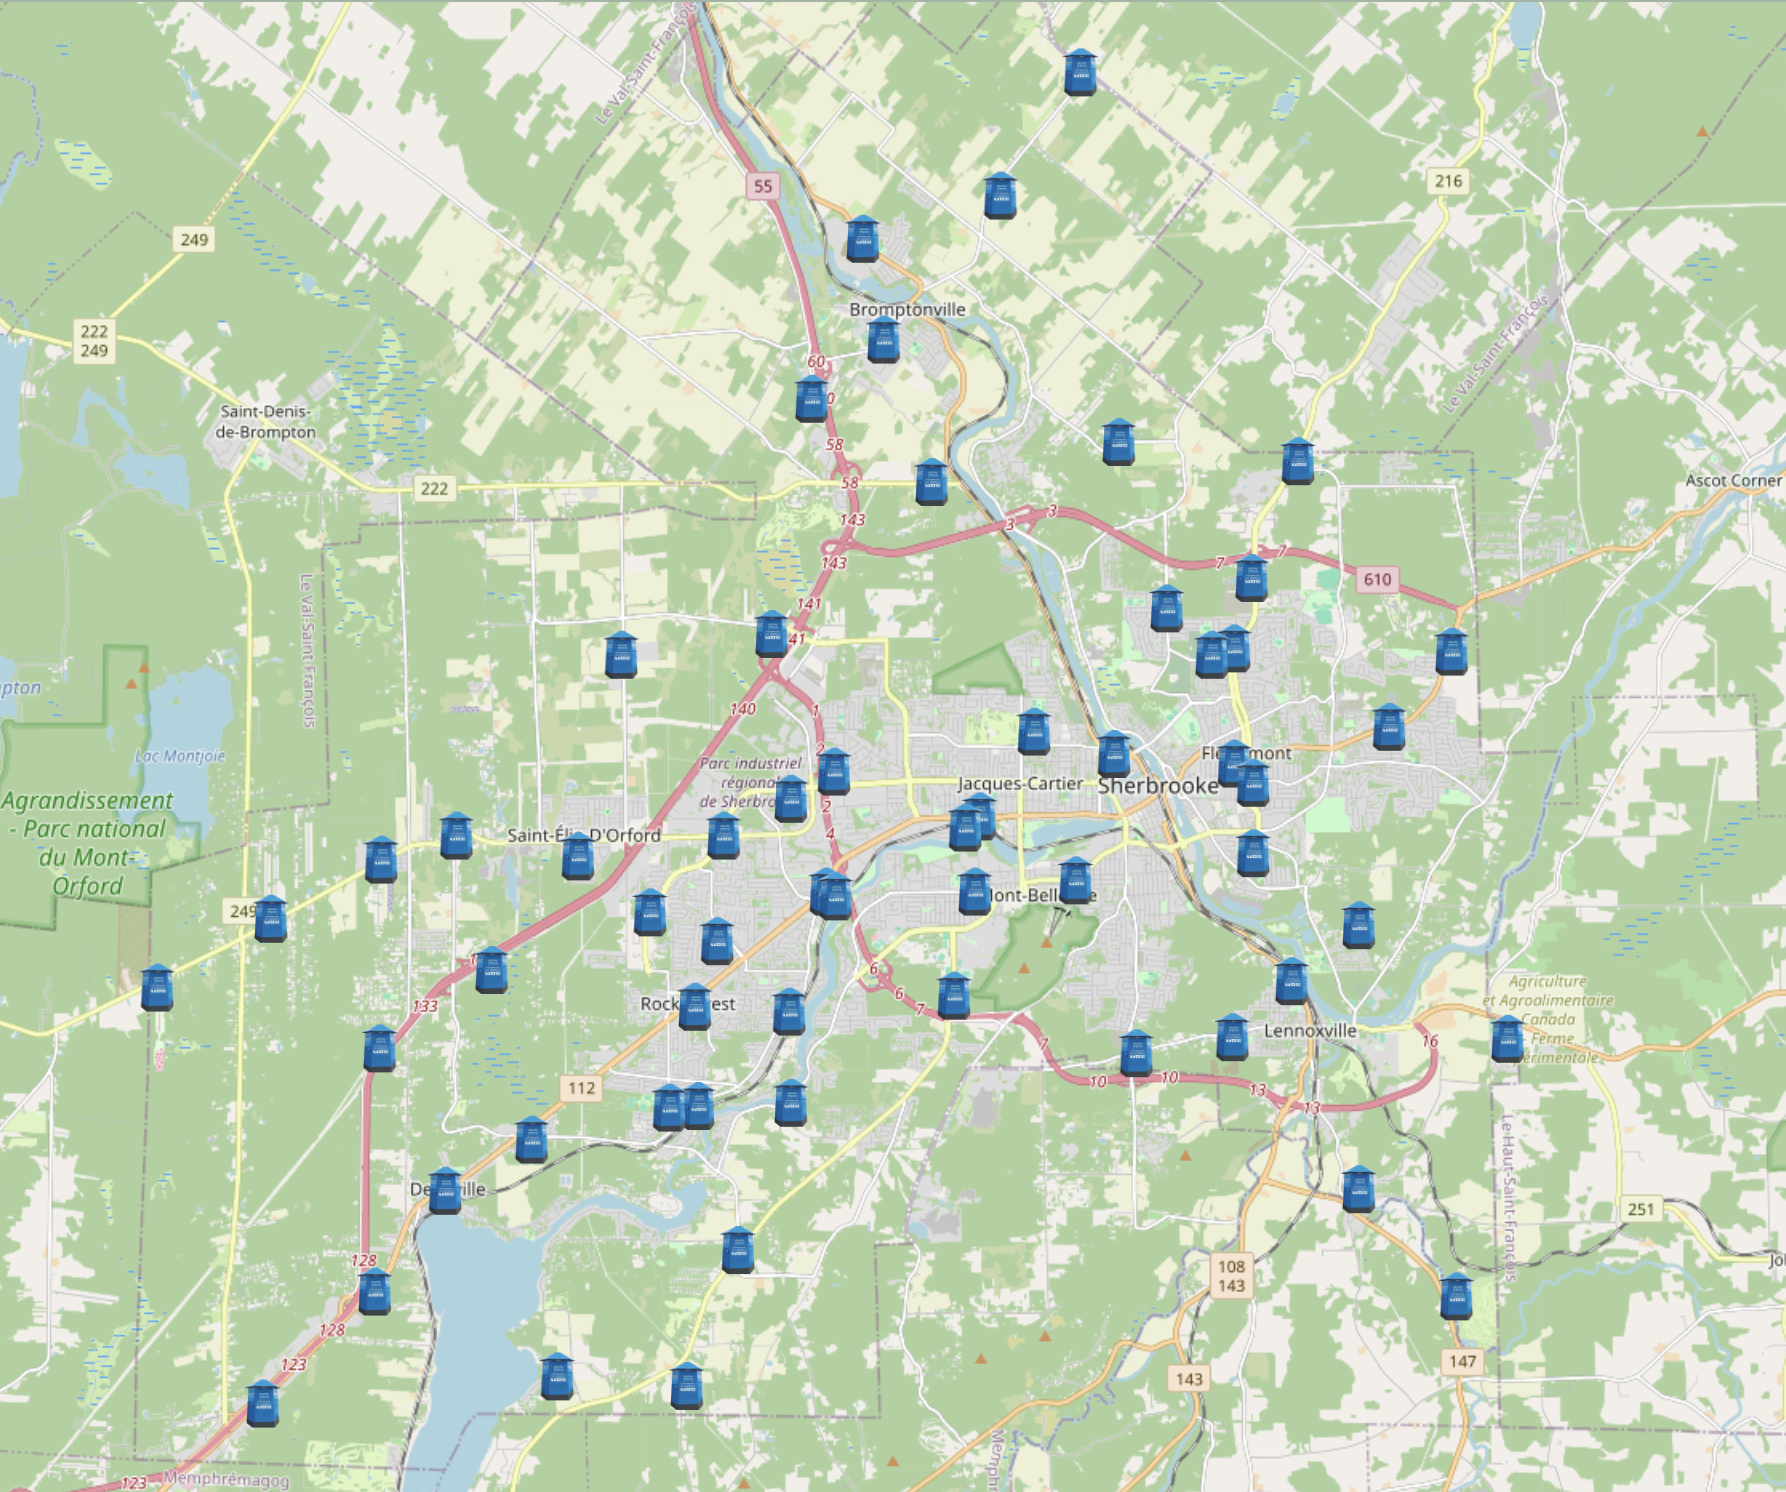
\includegraphics[width=0.30\linewidth]{images/new_quantum.png}
    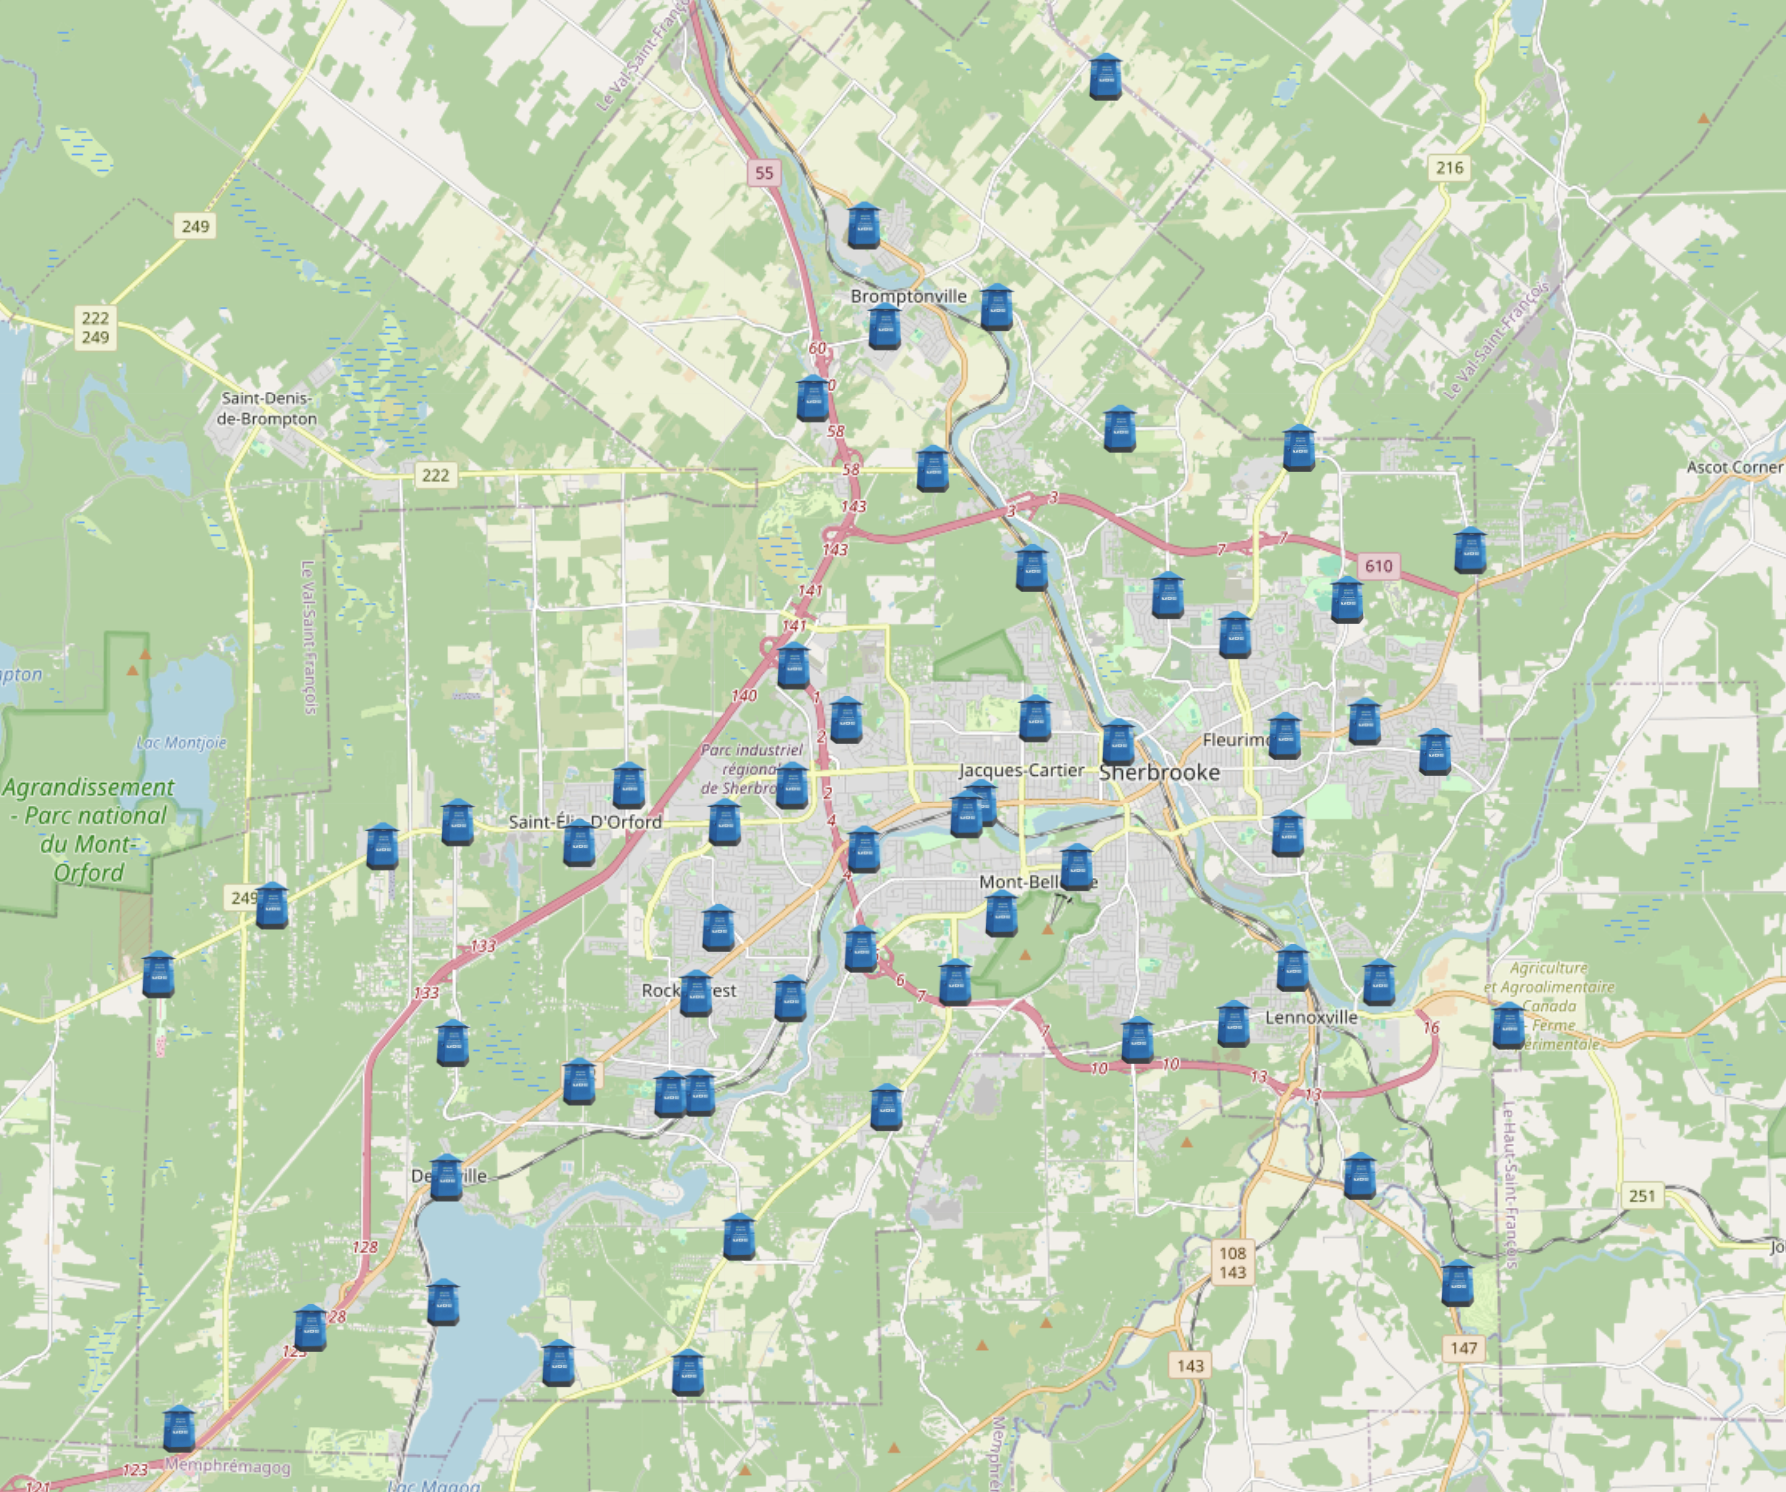
\includegraphics[width=0.30\linewidth]{images/new_classical.png}
    \caption{À gauche, la répartition originale des bacs. Au centre, la répartition obtenue avec la méthode quantique. À droite, la répartition obtenue avec la méthode classique.}
    \label{new_dist}
\end{figure}

\end{document}